\documentclass[11pt]{article}
 
\usepackage{hyperref}
\usepackage[T1]{fontenc}
\usepackage[polish]{babel}
\usepackage[utf8]{inputenc}
\usepackage{lmodern}
\usepackage{indentfirst}
\usepackage{caption}
\usepackage{amsmath}
\usepackage{lscape}
\usepackage{adjustbox}
\selectlanguage{polish}


\begin{document}

%----------------------------------------------------------------------------------------
%	Strona Tytułowa
%----------------------------------------------------------------------------------------

\begin{titlepage}

	\newcommand{\HRule}{\rule{\linewidth}{0.5mm}}
	
	\center
	
	%------------------------------------------------
	%	Nagłówki
	%------------------------------------------------
	
	\textsc{\LARGE \textbf{Uniwersytet Przyrodniczy we Wrocławiu}}\\[1cm] 
	
	\textsc{\Large Wydział Biologii i Hodowli Zwierząt}\\[0.5cm] 
	
	\textsc{\large Kierunek: Bioinformatyka}\\[0.5cm] 
	
	\textsc{\large Specjalność: Biostatystyka i programowanie bioinformatyczne}\\[0.5cm]
	
	\textsc{\large Przedmiot: Zaawansowane elementy stosowania pakietów statystycznych}\\[0.5cm]
	
	%------------------------------------------------
	%	Tytuł
	%------------------------------------------------
	
	\HRule\\[0.4cm]
	
	{\huge\bfseries Analiza oraz modelowanie łącznej kwoty odrzuconych pożyczek na podstawie raportu Lending Club w latach 2007-2012}\\[0.4cm] 
	
	\HRule\\[1.5cm]
	
	%------------------------------------------------
	%	Autor
	%------------------------------------------------
	
	\begin{minipage}{0.4\textwidth}
		\begin{flushleft}
			\large
			\textit{Autor}\\
			Artur \textsc{Wójtowicz}
		\end{flushleft}
	\end{minipage}
	~
	\begin{minipage}{0.4\textwidth}
		\begin{flushright}
			\large
			\textit{Prowadzący}\\
			dr inż. Anna \textsc{Mucha} % Prowadzący
		\end{flushright}
	\end{minipage}
	
	
	\vfill\vfill\vfill
	{\large\today}
	\vfill 
	
\end{titlepage}

%----------------------------------------------------------------------------------------
\newpage

\tableofcontents

\newpage

\section{Wprowadzenie}

\subsection{Zbiór danych}
Dane, które zostały użyte w tym sprawozdaniu, pochodzą z głównej strony firmy \textit{Lending Club} - firmy będącej pośrednikiem między pożyczkodawcą a pożyczkobiorcą na terenie USA, zaś dane, są ogólnodostępne na oficjalnej stronie, pod adresem:
\begin{center}
\url{https://www.lendingclub.com/info/download-data.action}
\end{center}

Zbiór danych zawiera ponad 755 tysięcy rekordów odrzuconych pożyczek w latach od 26 maja 2007 do 31 grudnia 2012 oraz dziewięć kolumn, na które składają się:
\begin{itemize}
\item \textit{Amount Requested} - Kwota całkowita wnioskowana przez pożyczkobiorcę;
\item \textit{Application Date} - Data aplikacji o pożyczkę przez pożyczkobiorcę;
\item \textit{Loan Title} - Tytuł pożyczki podaną przez pożyczkobiorcę;
\item \textit{Risk Score} - Do 5 listopada 2013 używano tutaj \textit{FICO score} stworzonego przez \textit{Fair Isaac Corporation} do oceny ryzyka udzielenia pożyczki. Po 5 listopada 2013 roku, do oceny ryzyka korzystano z Vantage score;
\item \textit{Debt-To-Income Ratio} - Obliczona proporcja względem całkowitych miesięcznych spłat zadłużeń pożyczkodawcy, odliczając od tego zakwaterowanie i wnioskowaną pożyczkę. Wartość ta, jest dzielona przez miesięczne przychody pożyczkobiorcy, które zgłosił;
\item \textit{Zip Code} - Pierwsze trzy numery kodu pocztowego pożyczkobiorcy;
\item \textit{State} - Stan (w USA), w którym pożyczkodawca składa aplikację o pożyczkę;
\item \textit{Employment Length} - Okres w latach zatrudnienia. Możliwe wartości znajdują się pomiędzy 0 a 10, gdzie 0 oznacza mniej niż rok zaś 10 więcej niż dziesięc lat.
\item \textit{Policy Code} - W przypadku naszych danych, wartość każdego rekordu tutaj, jest równa 0.
\end{itemize}

Do analiz szeregów czasowych, potrzebować będziemy jedynie dwóch pierwszych kolumn - \textit{Amount Requested} oraz \textit{Application Date}. W celu ich wyciągnięcia oraz dopasowania, napisany został skrypt w języku \textit{Python}, który tworzy dwa pliki csv. Pierwszy, zawierający dzienną sumę pożyczek wnioskowanych przez pożyczkobiorcę, oraz drugi, zawierający miesięczną sumę pożyczek wnioskowanych przez pożyczkobiorcę.

\begin{figure}[h]

    \centering
	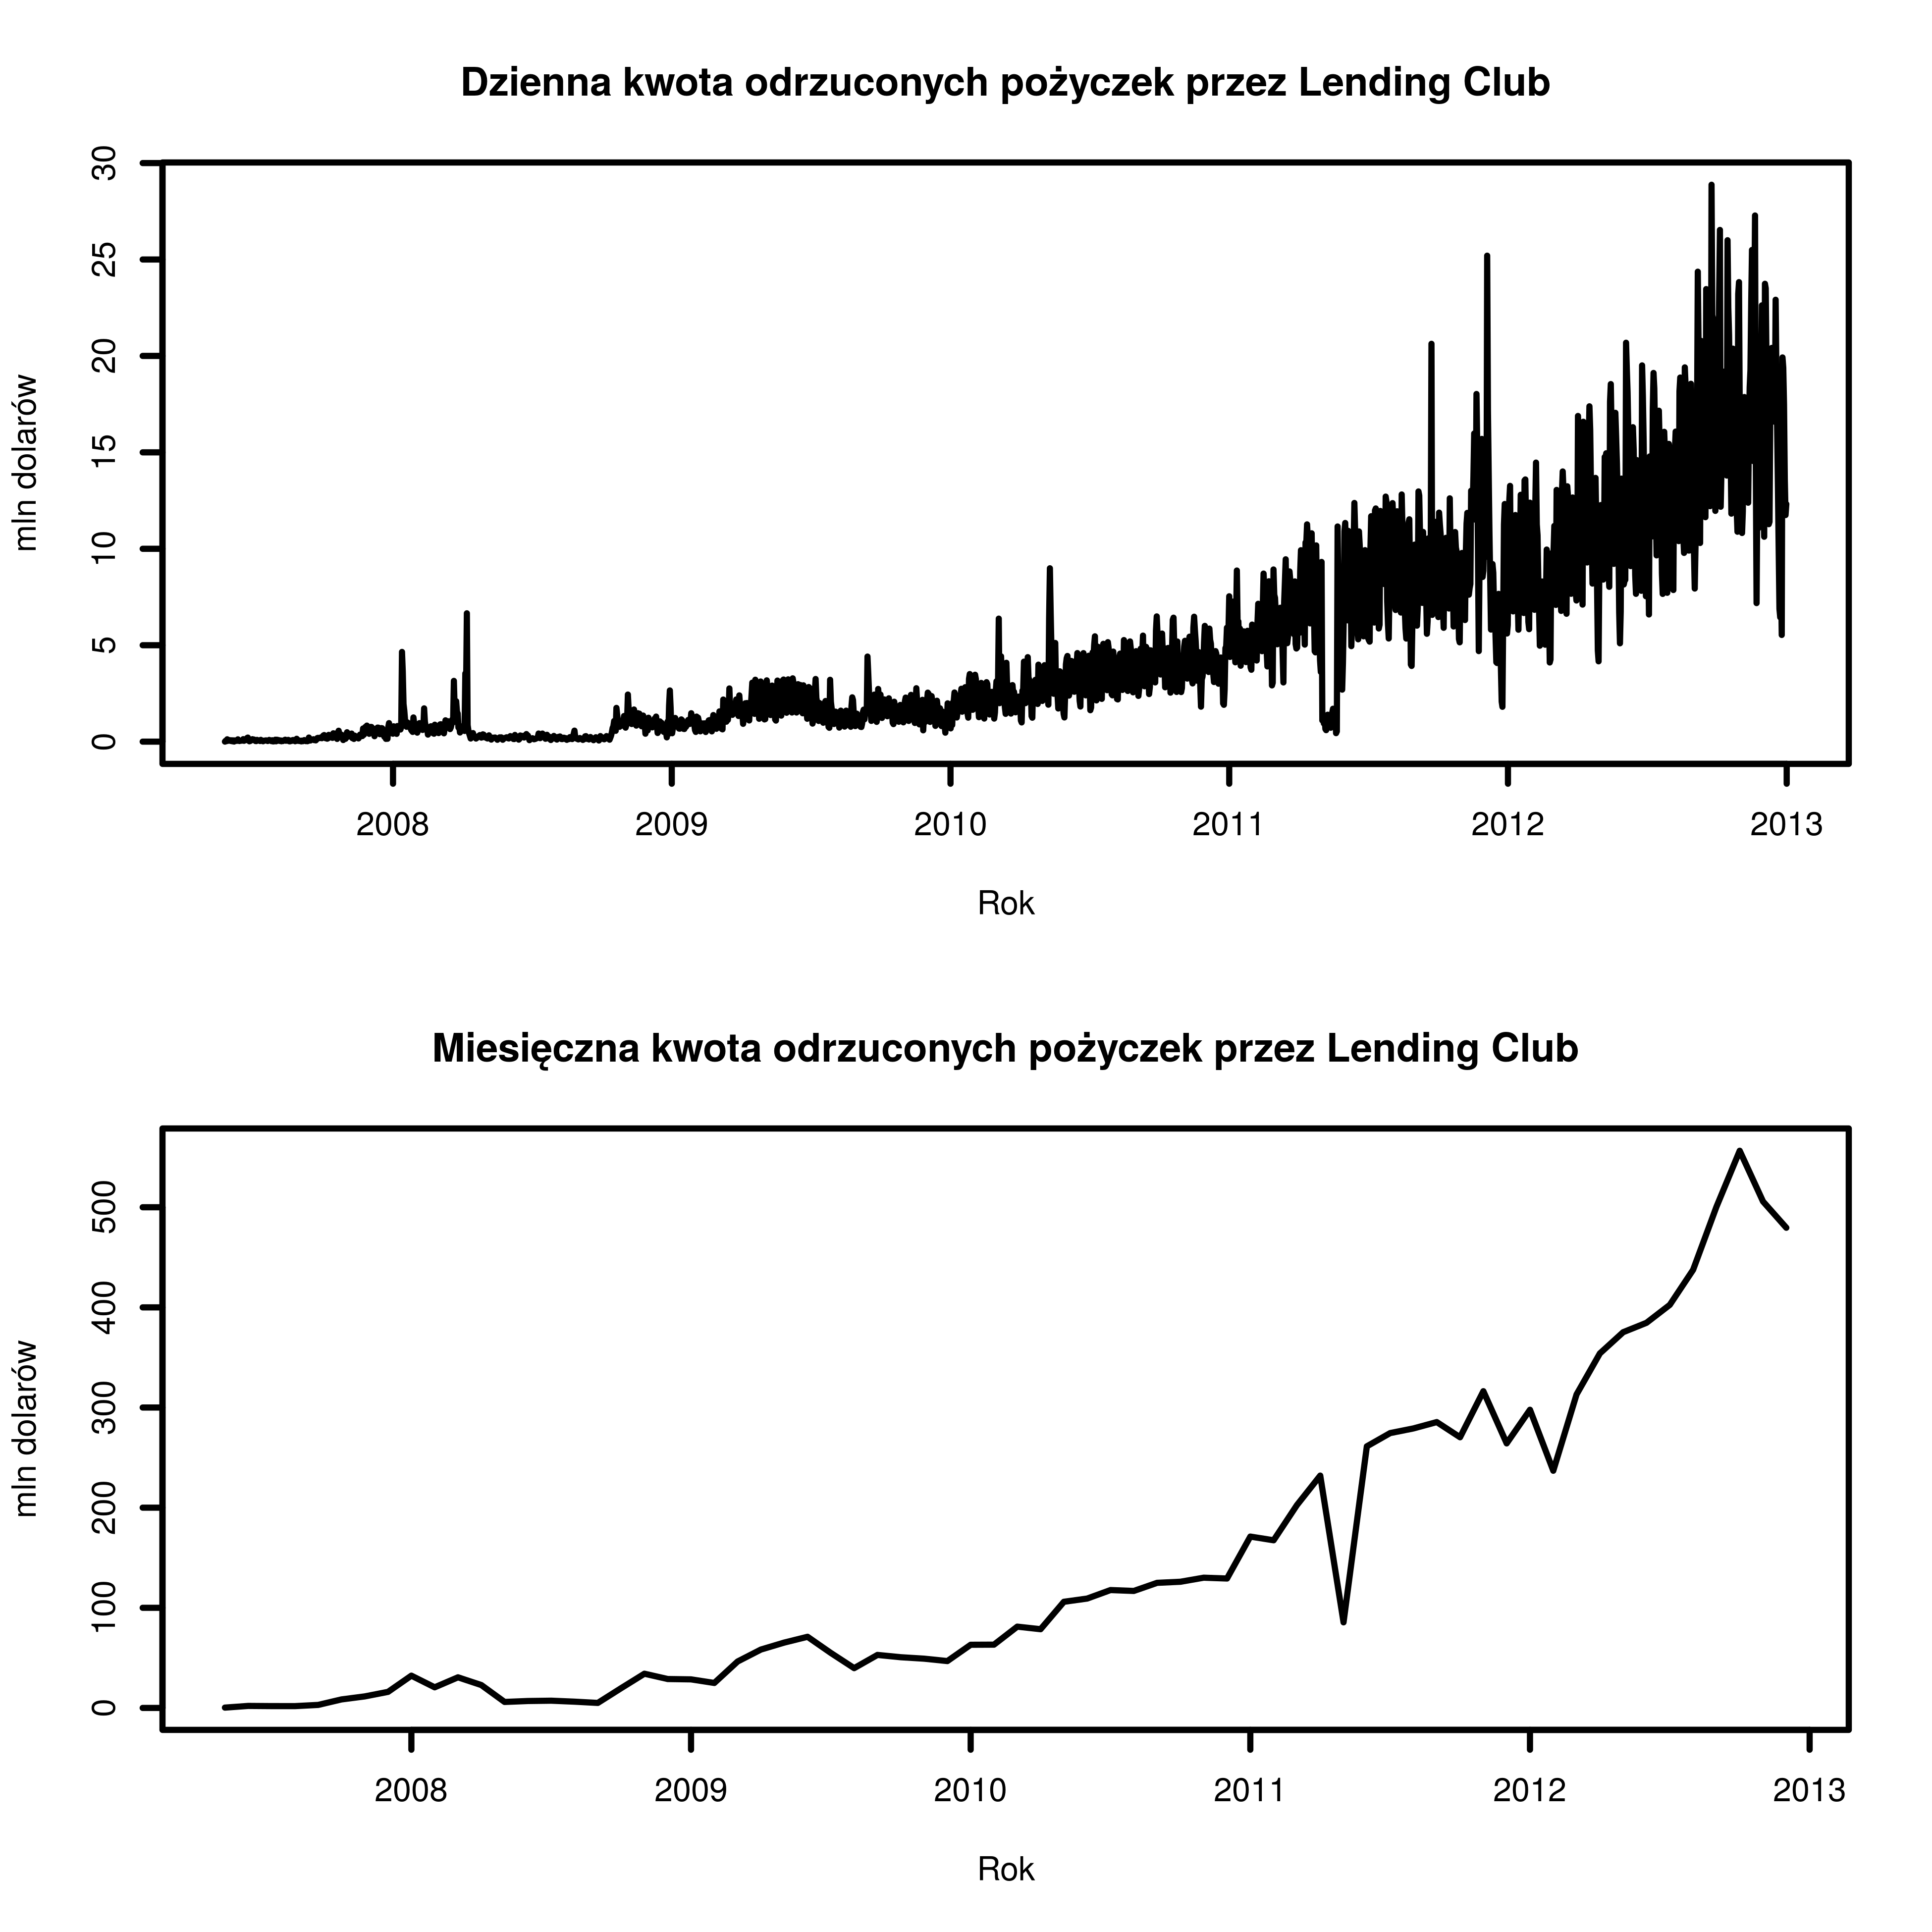
\includegraphics[width=\textwidth]{images/data_ogolnie_ts.png}
    \caption{Ogólne przedstawienie danych dziennych oraz miesięcznych w czasie.}
    \label{fig:data_ogolnie_ts}

\end{figure}

\newpage

Czyste dane zostały przedstawione na Rysunek \ref{fig:data_ogolnie_ts}, gdzie już na starcie możemy zauważyć trend wzrostowy. Problematyczny może tutaj się okazać miesiąc maj w roku 2011, gdzie widzimy intensywny spadek ilości odrzuconych pożyczek. Istnieje wiele przesłanek tak intensywnego spadku, jednakże najpewniejszymi są:
\begin{itemize}
\item Usunięcie lub awaria bazy danych;
\item Działanie na rzecz wykluczenia danych ogólnodostępnych;
\end{itemize}
Firma \textit{Lending Club} wystartowała na Facebooku w 2006 roku, a na giełdę wskoczyła dopiero 12 grudnia 2014, więc nie jesteśmy w stanie stwierdzić, czy występowało wtedy załamanie giełdowe dla tej firmy, stąd możliwe jedynie spekulacje dotyczące załamania tendencji wzrostowej.

Jednocześnie możemy zauważyć brak wzorców sezonowych w danych.

\subsection{Odstępstwa w danych}

Analiza, którą przeprowadzam będzie na niezmodyfikowanych danych udostępnionych przez \textit{Lending Club}, jednakże dobrze jest wiedzieć o odstępstwach w danych. Analizujemy dane jedynie odrzuconych pożyczek dla osób fizycznych.

\textit{Lending Club} oferuje pożyczki do 40 tysięcy dolarów dla osób prywatnych oraz do 300 tysięcy dolarów dla małych firm. Analizując bezpośrednio ogólnodostepne dane, możemy znaleźć dwa rekordy na wysokość pożyczki 0. Zauważyłem również, że istnieje kilkadziesiąt rekordów odstających wzwyż od zakładanych norm, dokładniej omówię sześć największych kwotowo aplikacji o pożyczkę:
\begin{itemize}
\item 10.09.2010 - 1.4 miliona dolarów na zakup samochodu;
\item 16.10.2012 - 1.2 miliona dolarów na konsolidację zadłużenia;
\item 16.10.2012 - milion dolarów na konsolidację zadłużenia
\item 09.06.2011 - 500 tysięcy dolarów na określony cel jako inne;
\item 15.06.2011 - 500 tysięcy dolarów na określony cel jako inne;
\item 22.08.2012 - 300 tysięcy dolarów na zakup samochód.
\end{itemize}

Jak możemy zauważyć, dwa z trzech zapytań o pożyczkę powyżej miliona dolarów miała miejsce tego samego dnia, na podobną kwotę. Możliwe jest, że była to ta sama osoba, która sprawdzała swoją zdolność kredytową po tym, jak zadłużyła się w innych firmach/bankach. Można to traktować jako dane nadmiarowe.

Podobną sytuację możemy zauważyć przy pożyczkach na 500 tysięcy dolarów, różnica dni pomiędzy nimi pozwala nam zakładać, że te zapytania zostały podane przez jedną osobę.

Pożyczki na 300 tysięcy lub 1.4 miliona dolarów na zakup samochodu, mogą wydawać się abstrakcyjne, jednakże jak powyżej, osoba wysyłająca zapytanie mogła sprawdzać jedynie swoją zdolność kredytową, lub pomylić się przy wypełnianiu aplikacji.

Analiza pozostałych czynników takich jak Risk Score, State, Debt-To-Income, przy bardzo podobnych pożyczkach jak wyżej wymieniłem może wskazywać na inną osobę, tak tym czynnikom nie należy wierzyć, ponieważ są one zależne od deklaracji pożyczkobiorcy. W zależności od Stanu, obowiązują inne przepisy. W zależności od deklaracji zarobkowych, mogą różnić się parametry Risk Score, Debt-To-Income. 

Łącznie cały zbiór zawiera 218 rekordów, w których kwota przekraczała 40 tysięcy dolarów. Chciałbym nadmienić, że 157 z tych rekordów, czyli 72\% miała przeznaczenie - zakup samochodu.
Po przeanalizowaniu odstępstw nasuwają mi się dwa wnioski:

\begin{itemize}
\item \textit{Lending Club} jest platformą internetową, każda osoba na wpół anonimowo może wypełnić wniosek w celu sprawdzenia swojej zdolności kredytowej. Zapytanie takie może być powielane przez jedną osobę dla wielu Stanów, deklaracji płacowych itd.;
\item Mógł wystąpić czynnik ludzki przy wypełnianiu wniosku o pożyczkę lub jego magazynowaniu;
\end{itemize}

\subsection{Kod źródłowy}

Kod źródłowy wszystkich omawianych skryptów napisanych w R oraz Python a także wszystkie rysunki dostępne są do pobrania na githubie. Link poniżej: 
\begin{center}
\url{https://github.com/arturwojtowicz/analiza_odrzuconych_pozyczek}
\end{center}

\newpage

\section{Wizualizacja i przekształcenia}

\subsection{Wykresy sezonowe}

Na wykresie pudełkowym widocznym na Rysunek \ref{fig:data_monthly_train_pudelkowy} możemy zauważyć spore różnice w średnich wartościach dla poszczególnych szeregów czasowych. Widzimy również załamanie w piątym miesiącu o czym wspominałem przy omawianiu Rysunek \ref{fig:data_ogolnie_ts}. Takiej samej informacji dostarczają nam pozostałe dwa wykresy - Rysunek  \ref{fig:data_monthly_train_sezonowy_ogolny}, \ref{fig:data_monthly_train_miesieczny_ogolny}. Zauważalny jest trend wzrostowy. Wahania sezonowe nie są widoczne.

\begin{figure}[h]

    \centering
	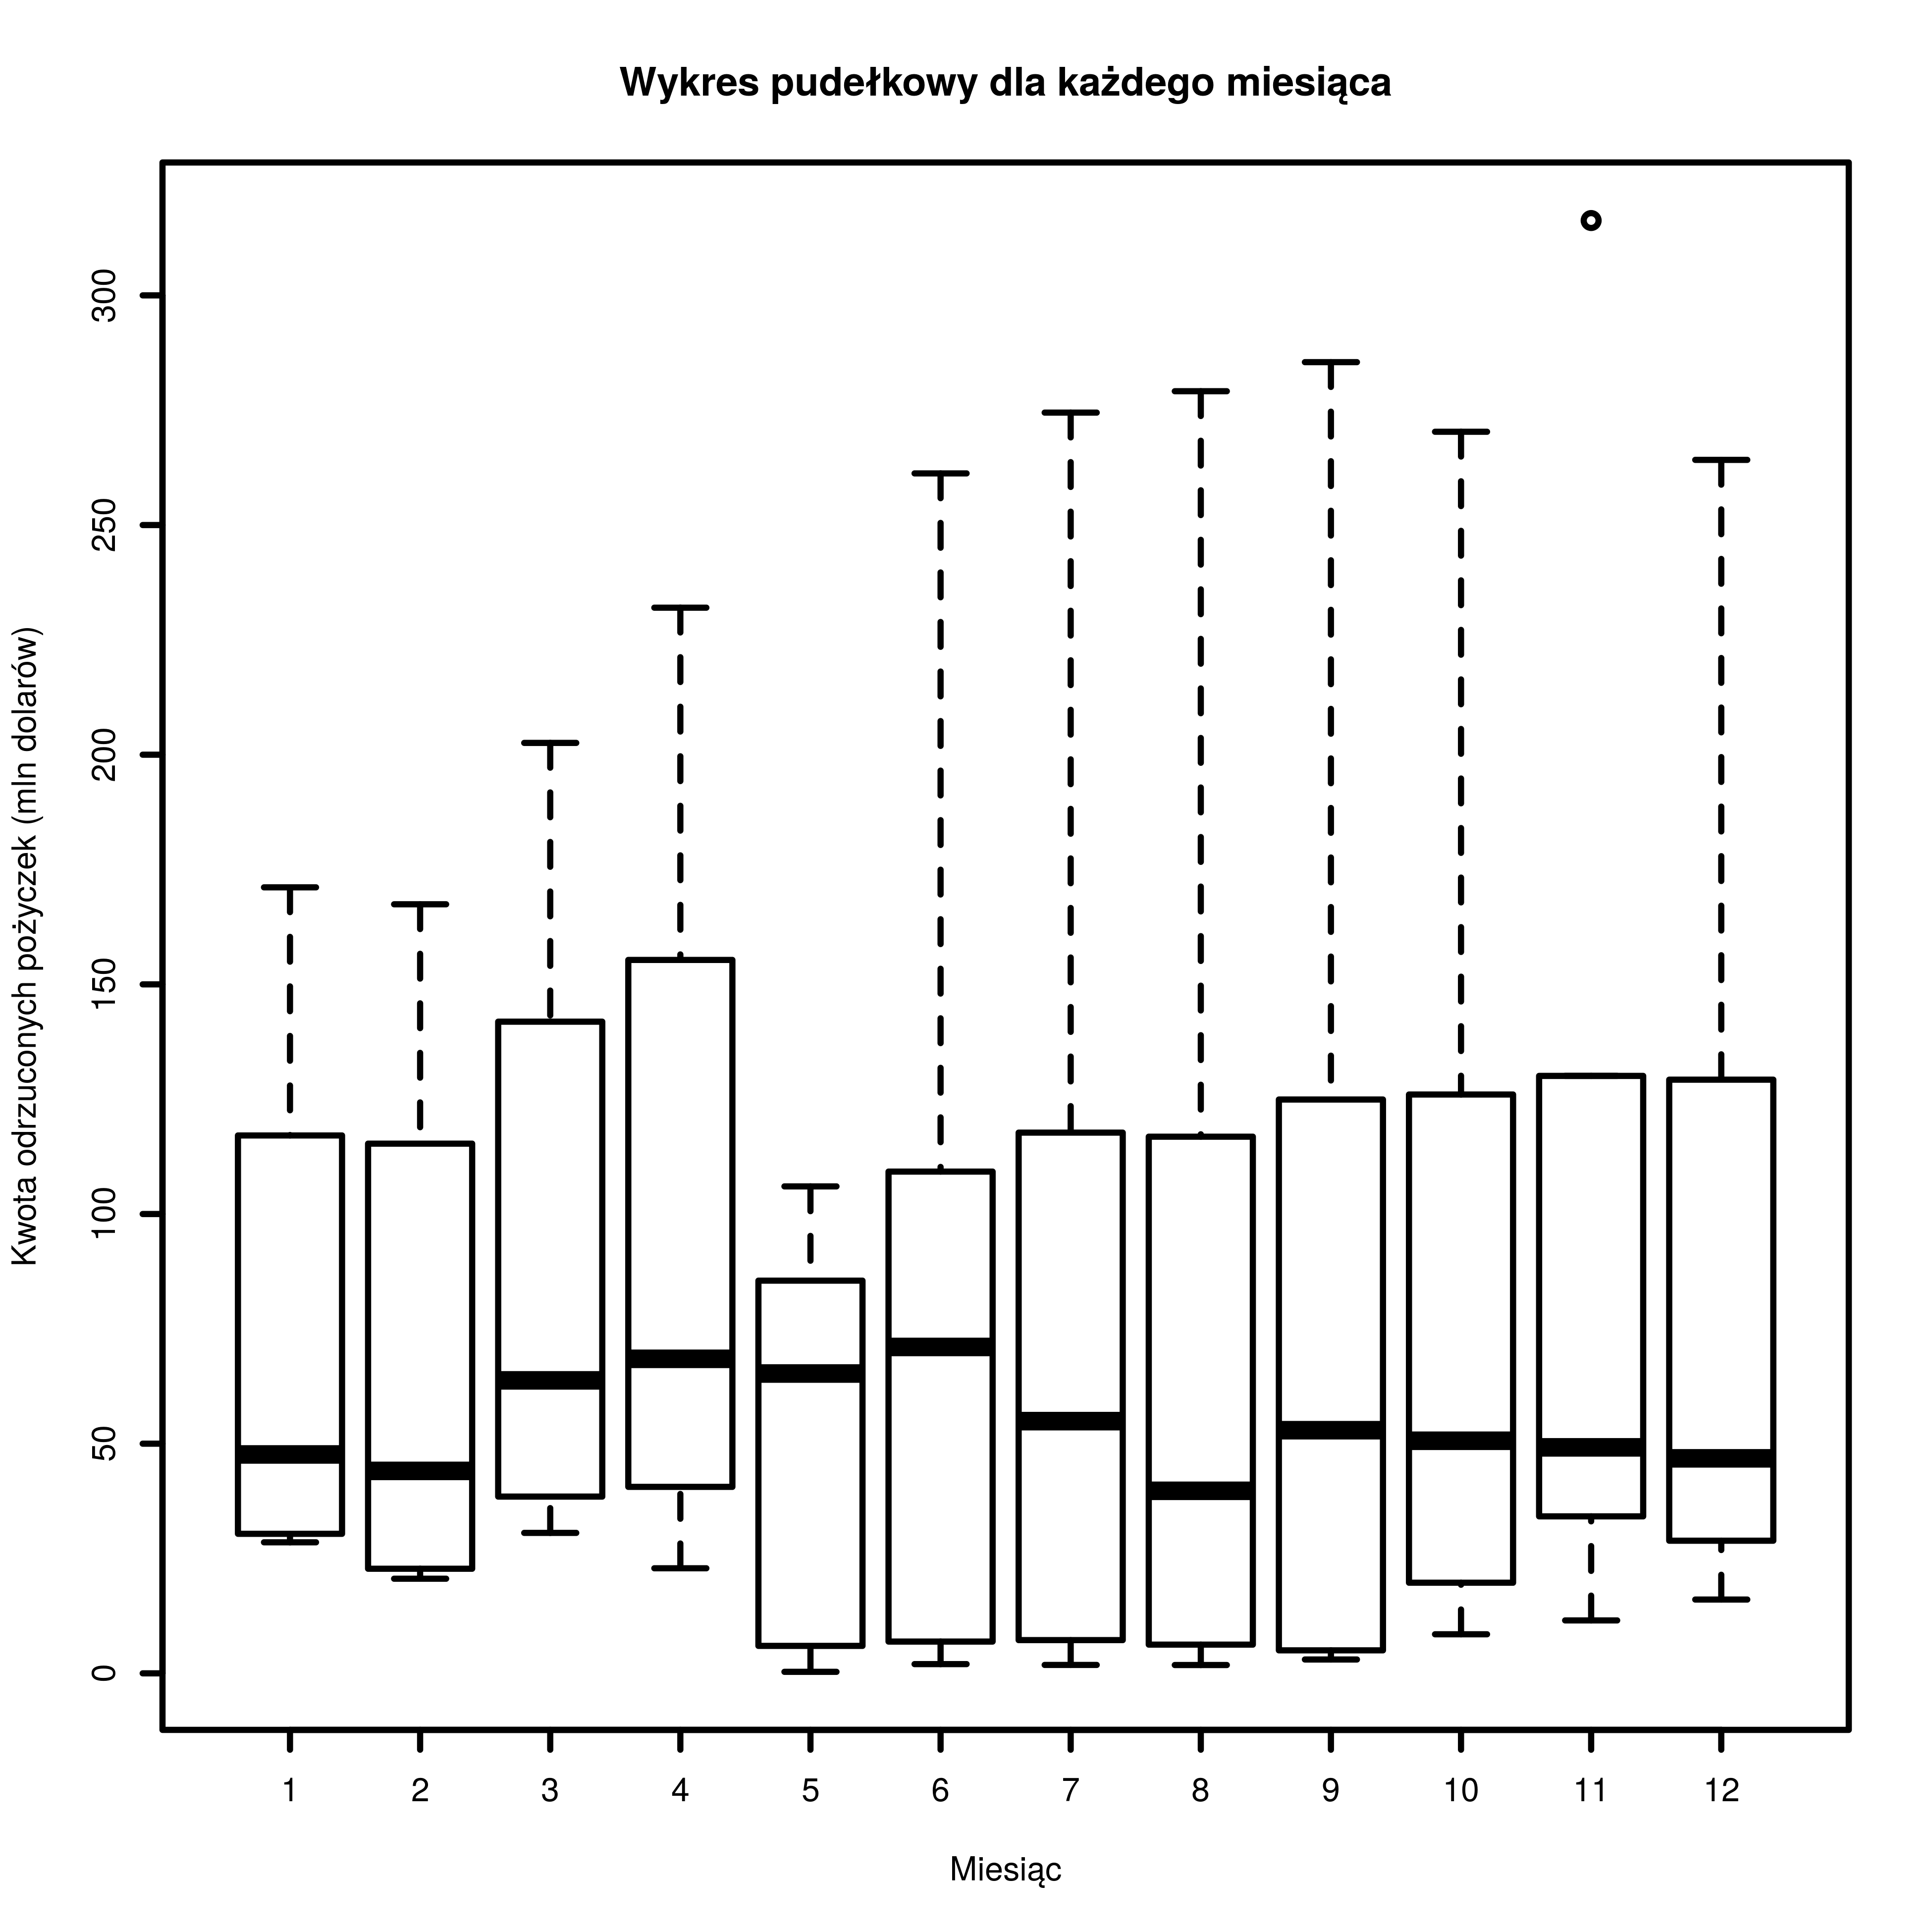
\includegraphics[width=\textwidth]{images/data_monthly_train_pudelkowy.png}
    \caption{Wykres pudełkowy każdego miesiąca dla analizowanego szeregu czasowego}
    \label{fig:data_monthly_train_pudelkowy}

\end{figure}

\newpage

\begin{figure}[h]

    \centering
	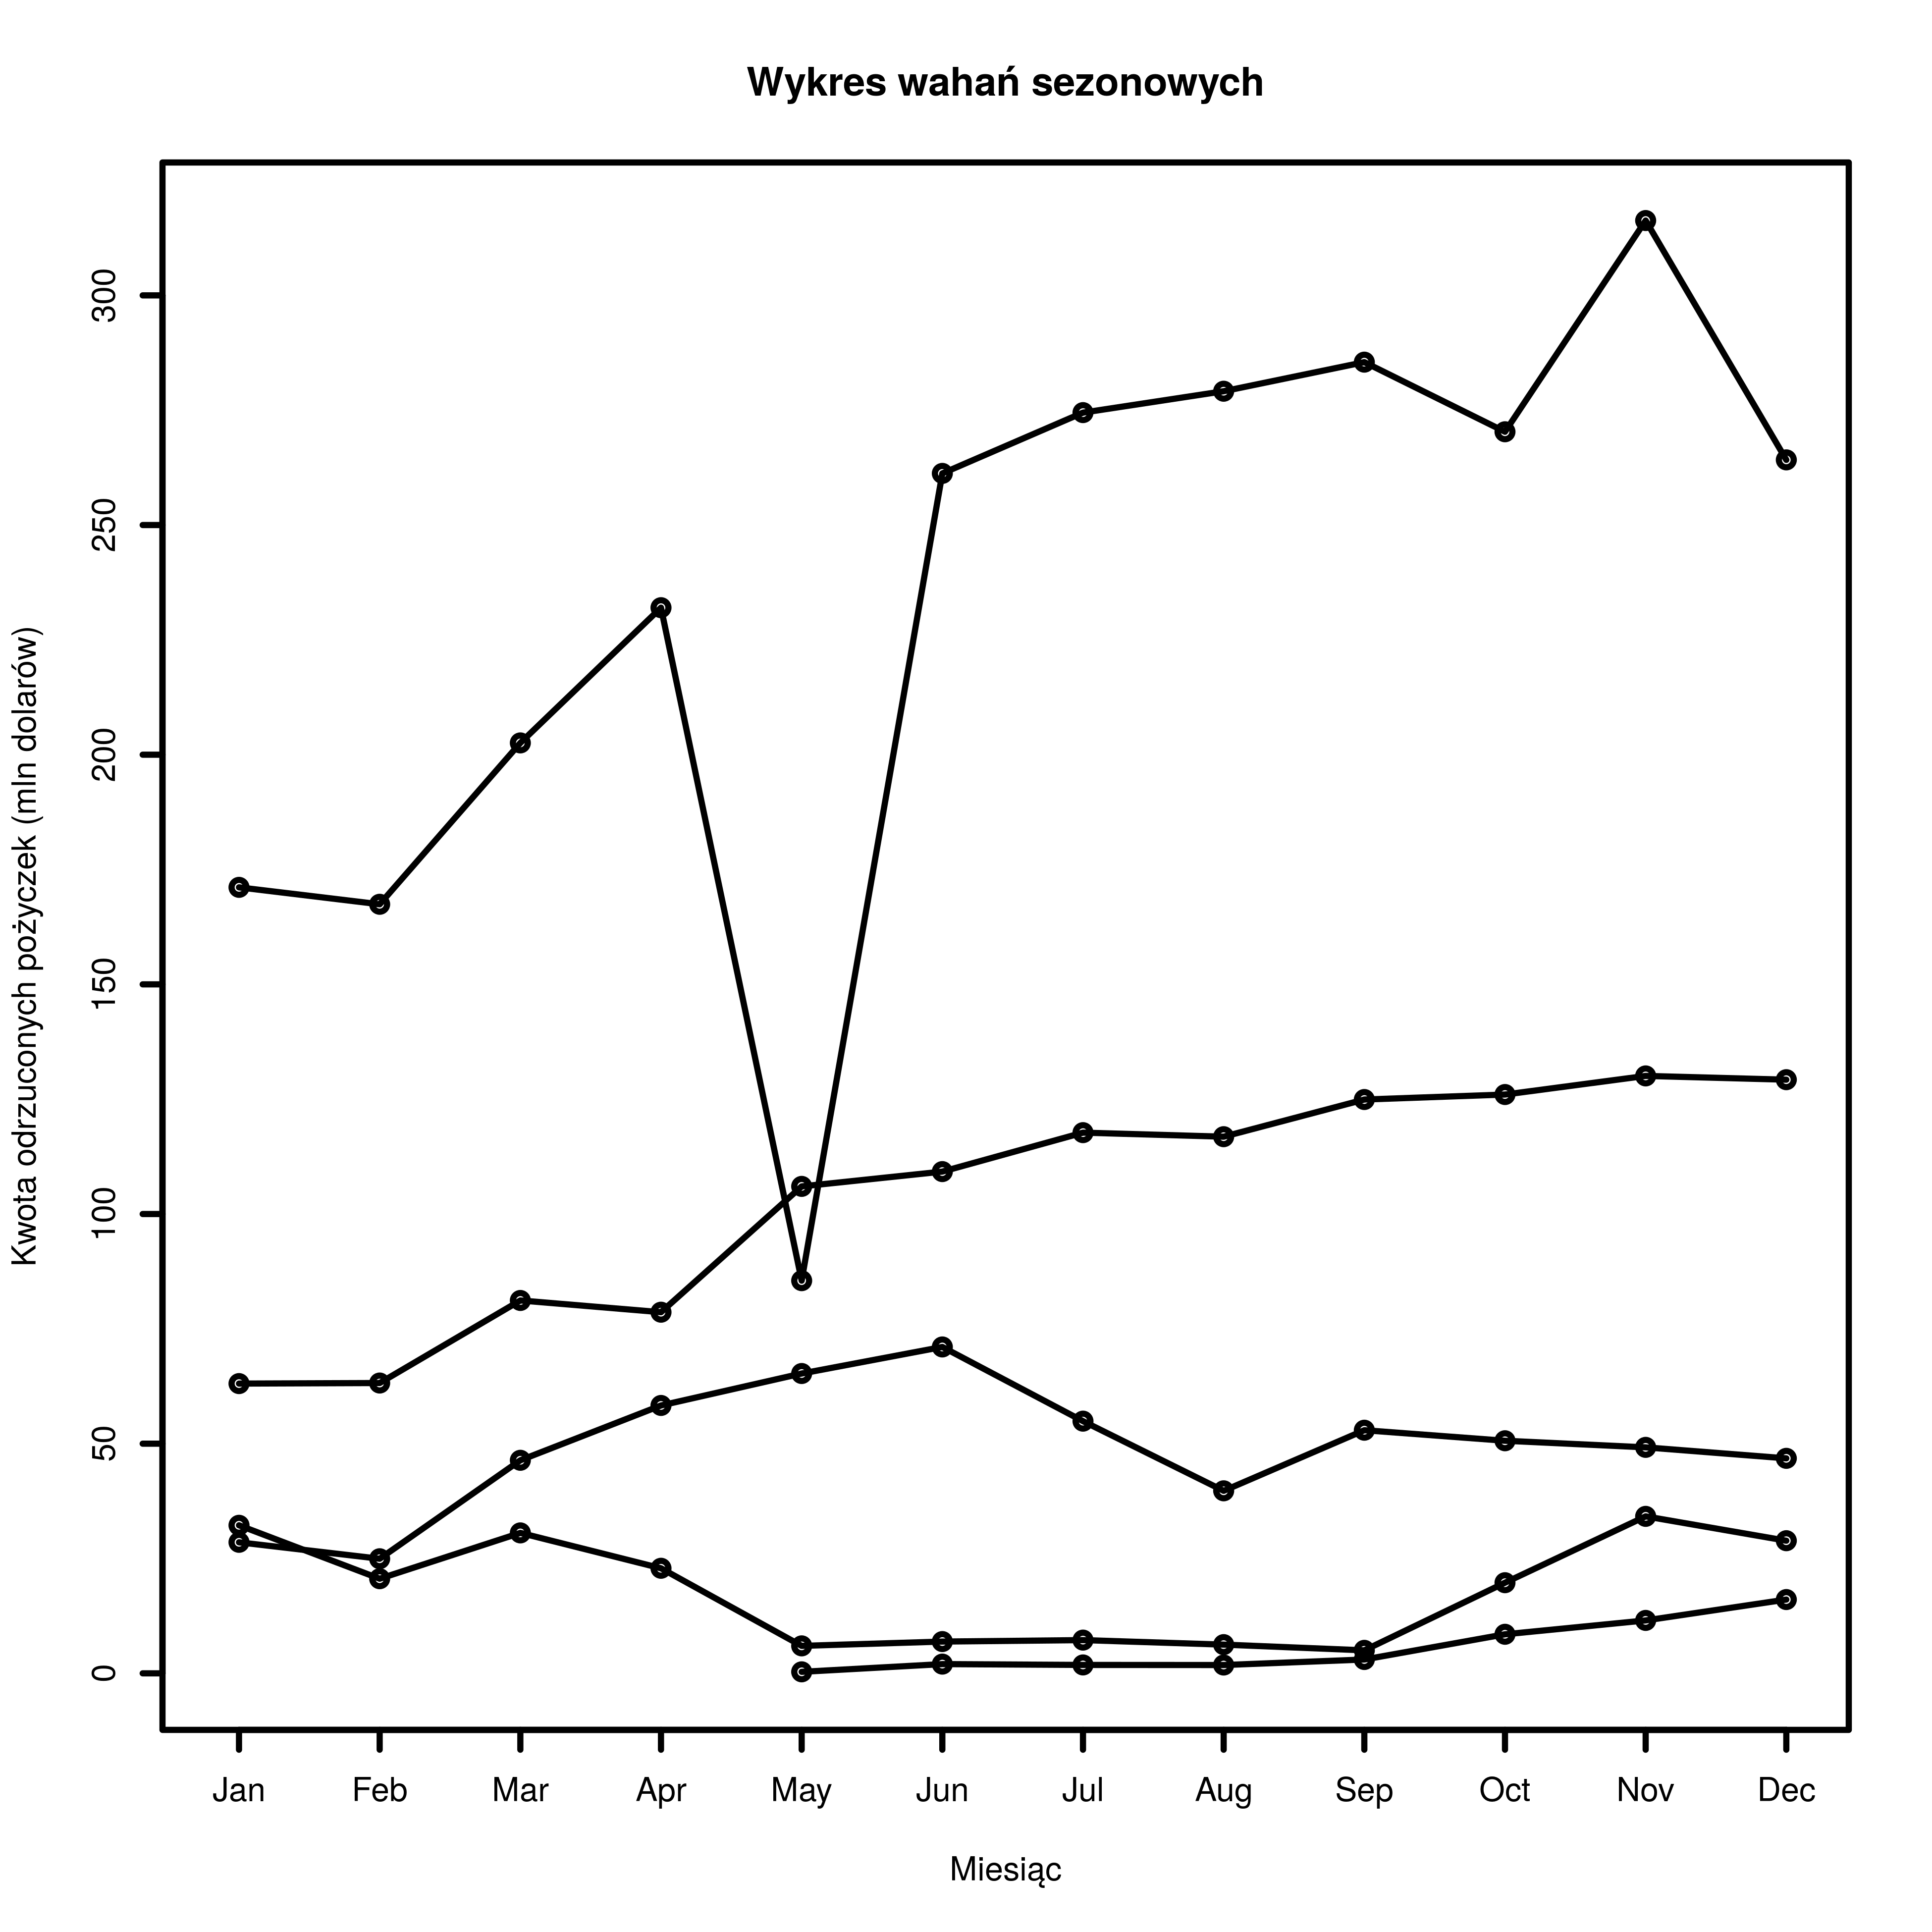
\includegraphics[width=\textwidth]{images/data_monthly_train_sezonowy_ogolny.png}
    \caption{Wykres wahań sezonowych każdego miesiąca dla analizowanego szeregu czasowego.}
    \label{fig:data_monthly_train_sezonowy_ogolny}

\end{figure}

\newpage

\begin{figure}[h]

    \centering
	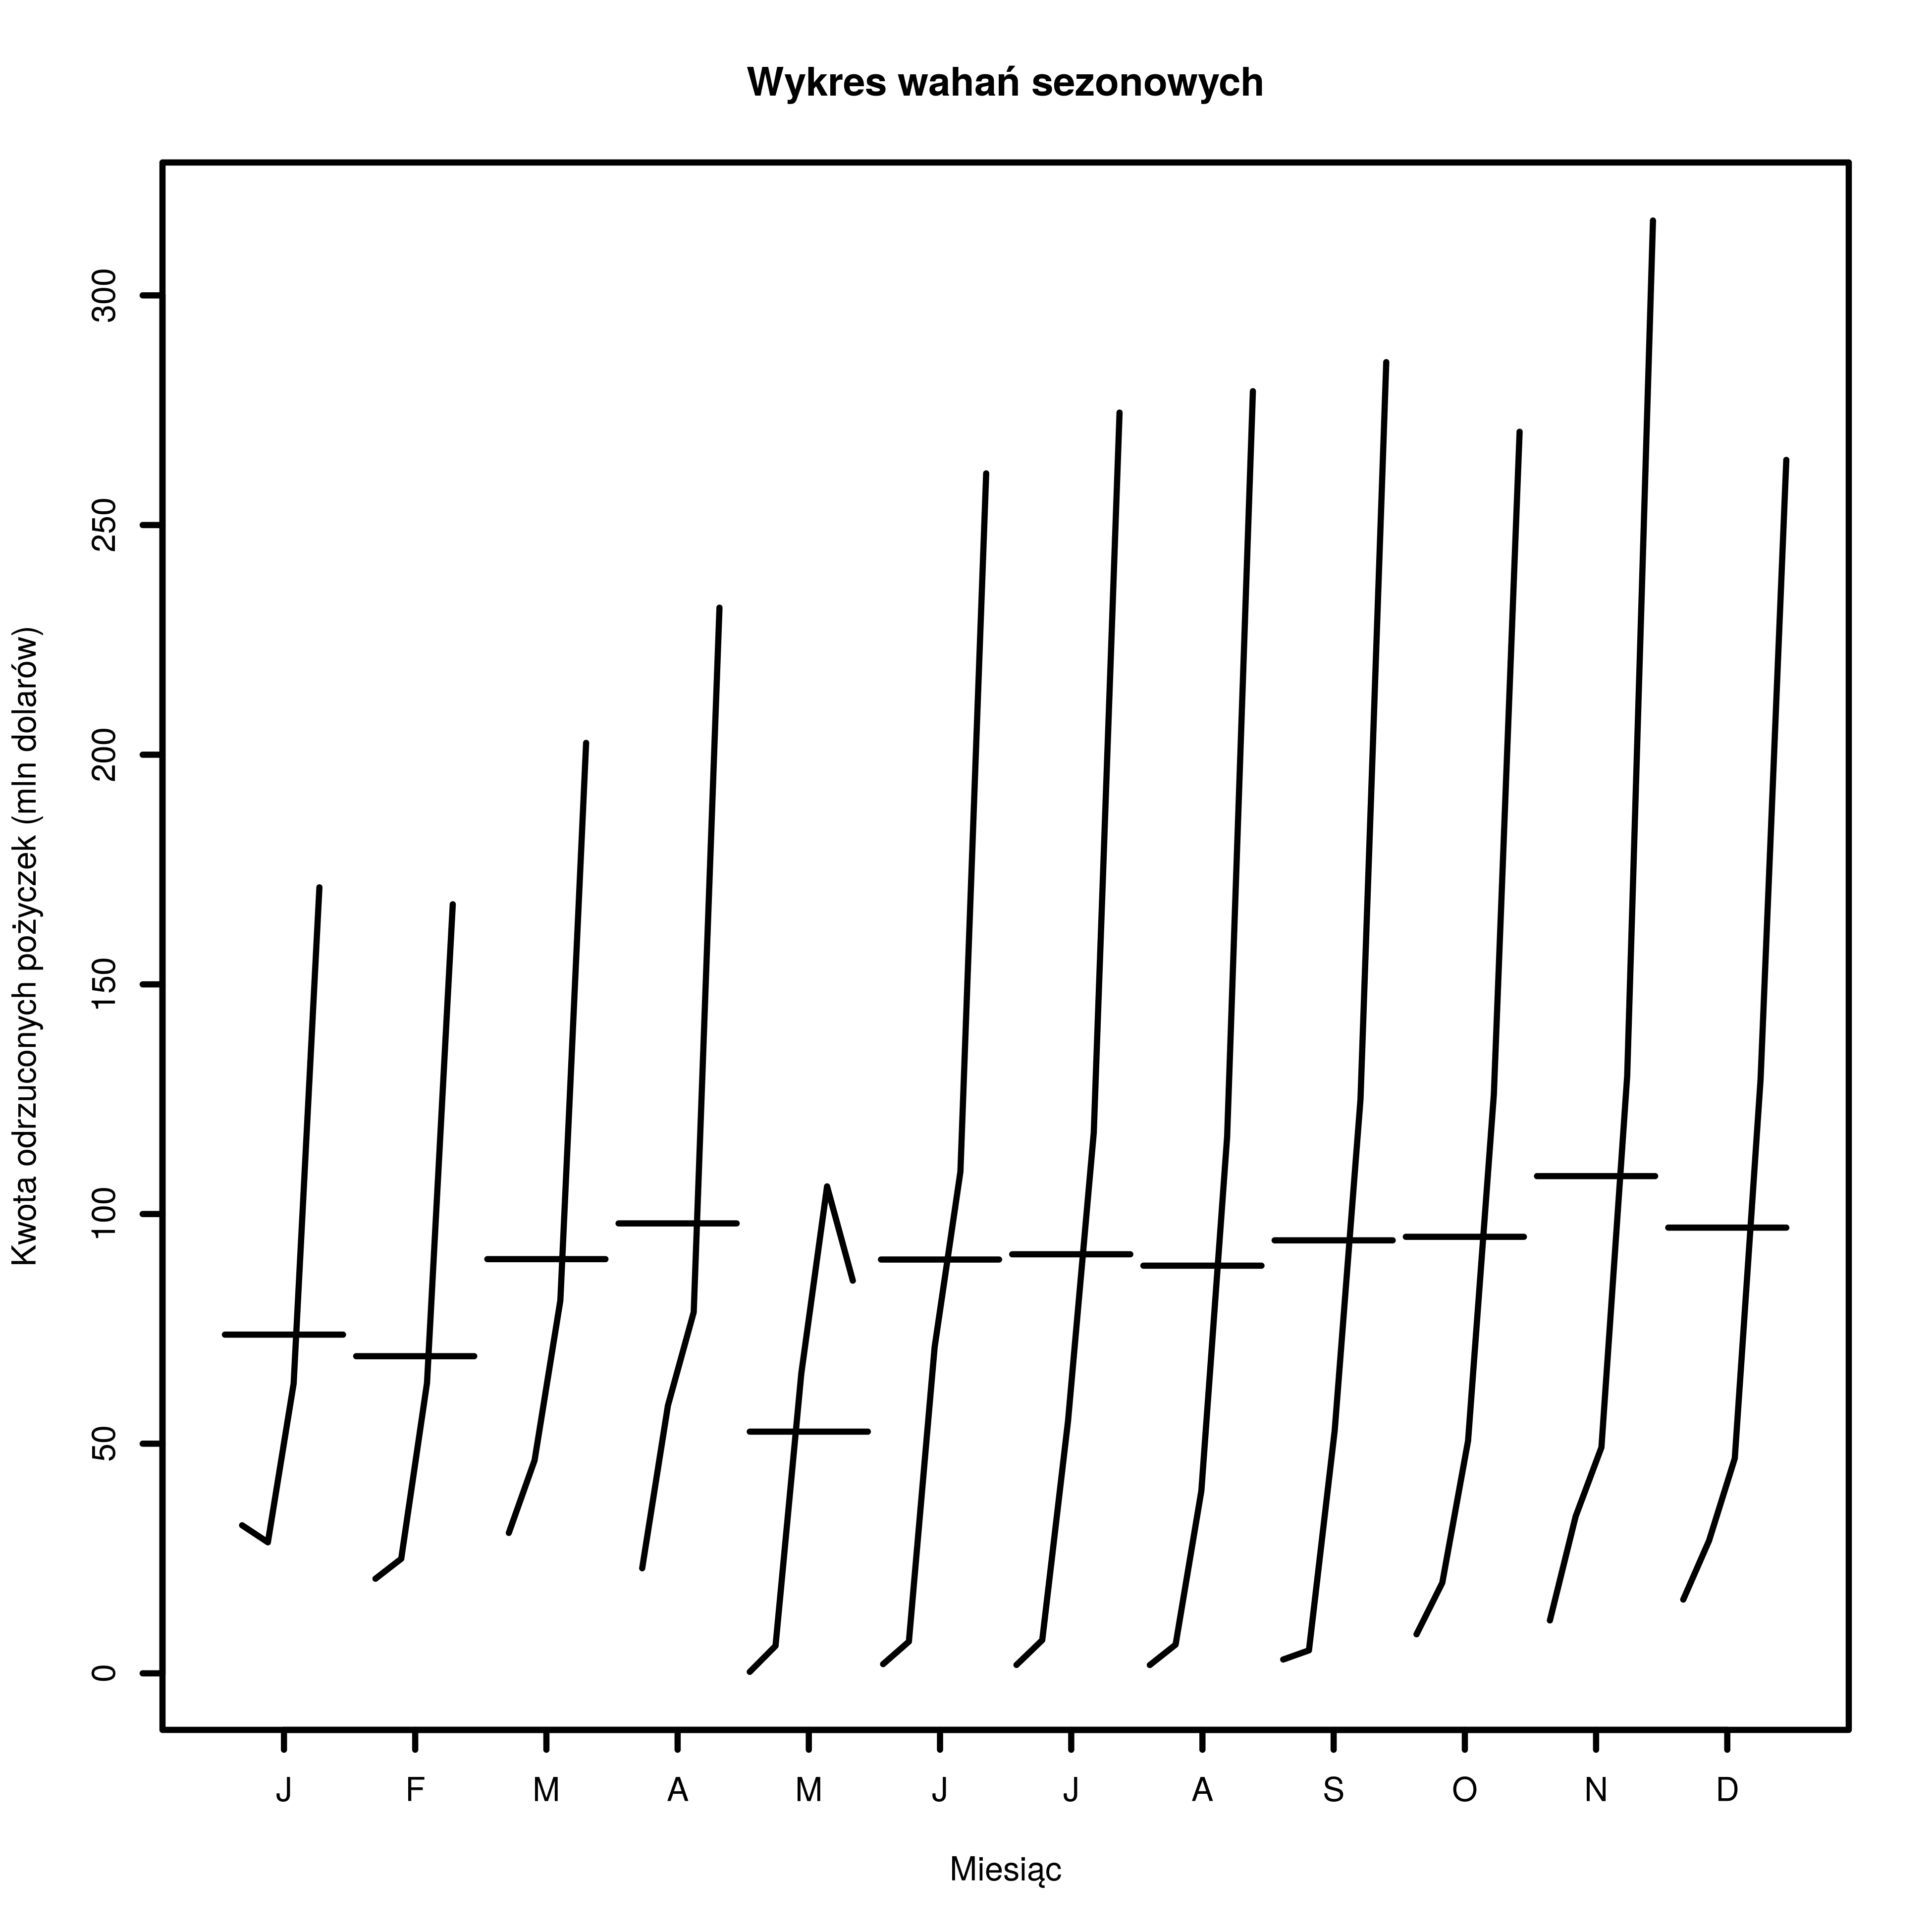
\includegraphics[width=\textwidth]{images/data_monthly_train_miesieczny_ogolny.png}
    \caption{Wykres wahań miesięcznych dla analizwanego szeregu czasowego.}
    \label{fig:data_monthly_train_miesieczny_ogolny}

\end{figure}

\newpage

\subsection{Wykresy autokorelacji}

Poniżej widzimy wykres rozrzutu dla wartości opóźnionych danych miesięcznych analizowanego szeregu czasowego. Jak możemy zauważyć dla opóźnienia 1 mamy silną korelację czasową, co oznacza, że trend rzeczywiście istnieje. Analizując opóźnienie 12, widzimy, że liniowość nie jest zachowana, przez co mamy kolejną przesłankę do wykluczenia sezonowości w naszych danych.

\begin{figure}[h]

    \centering
	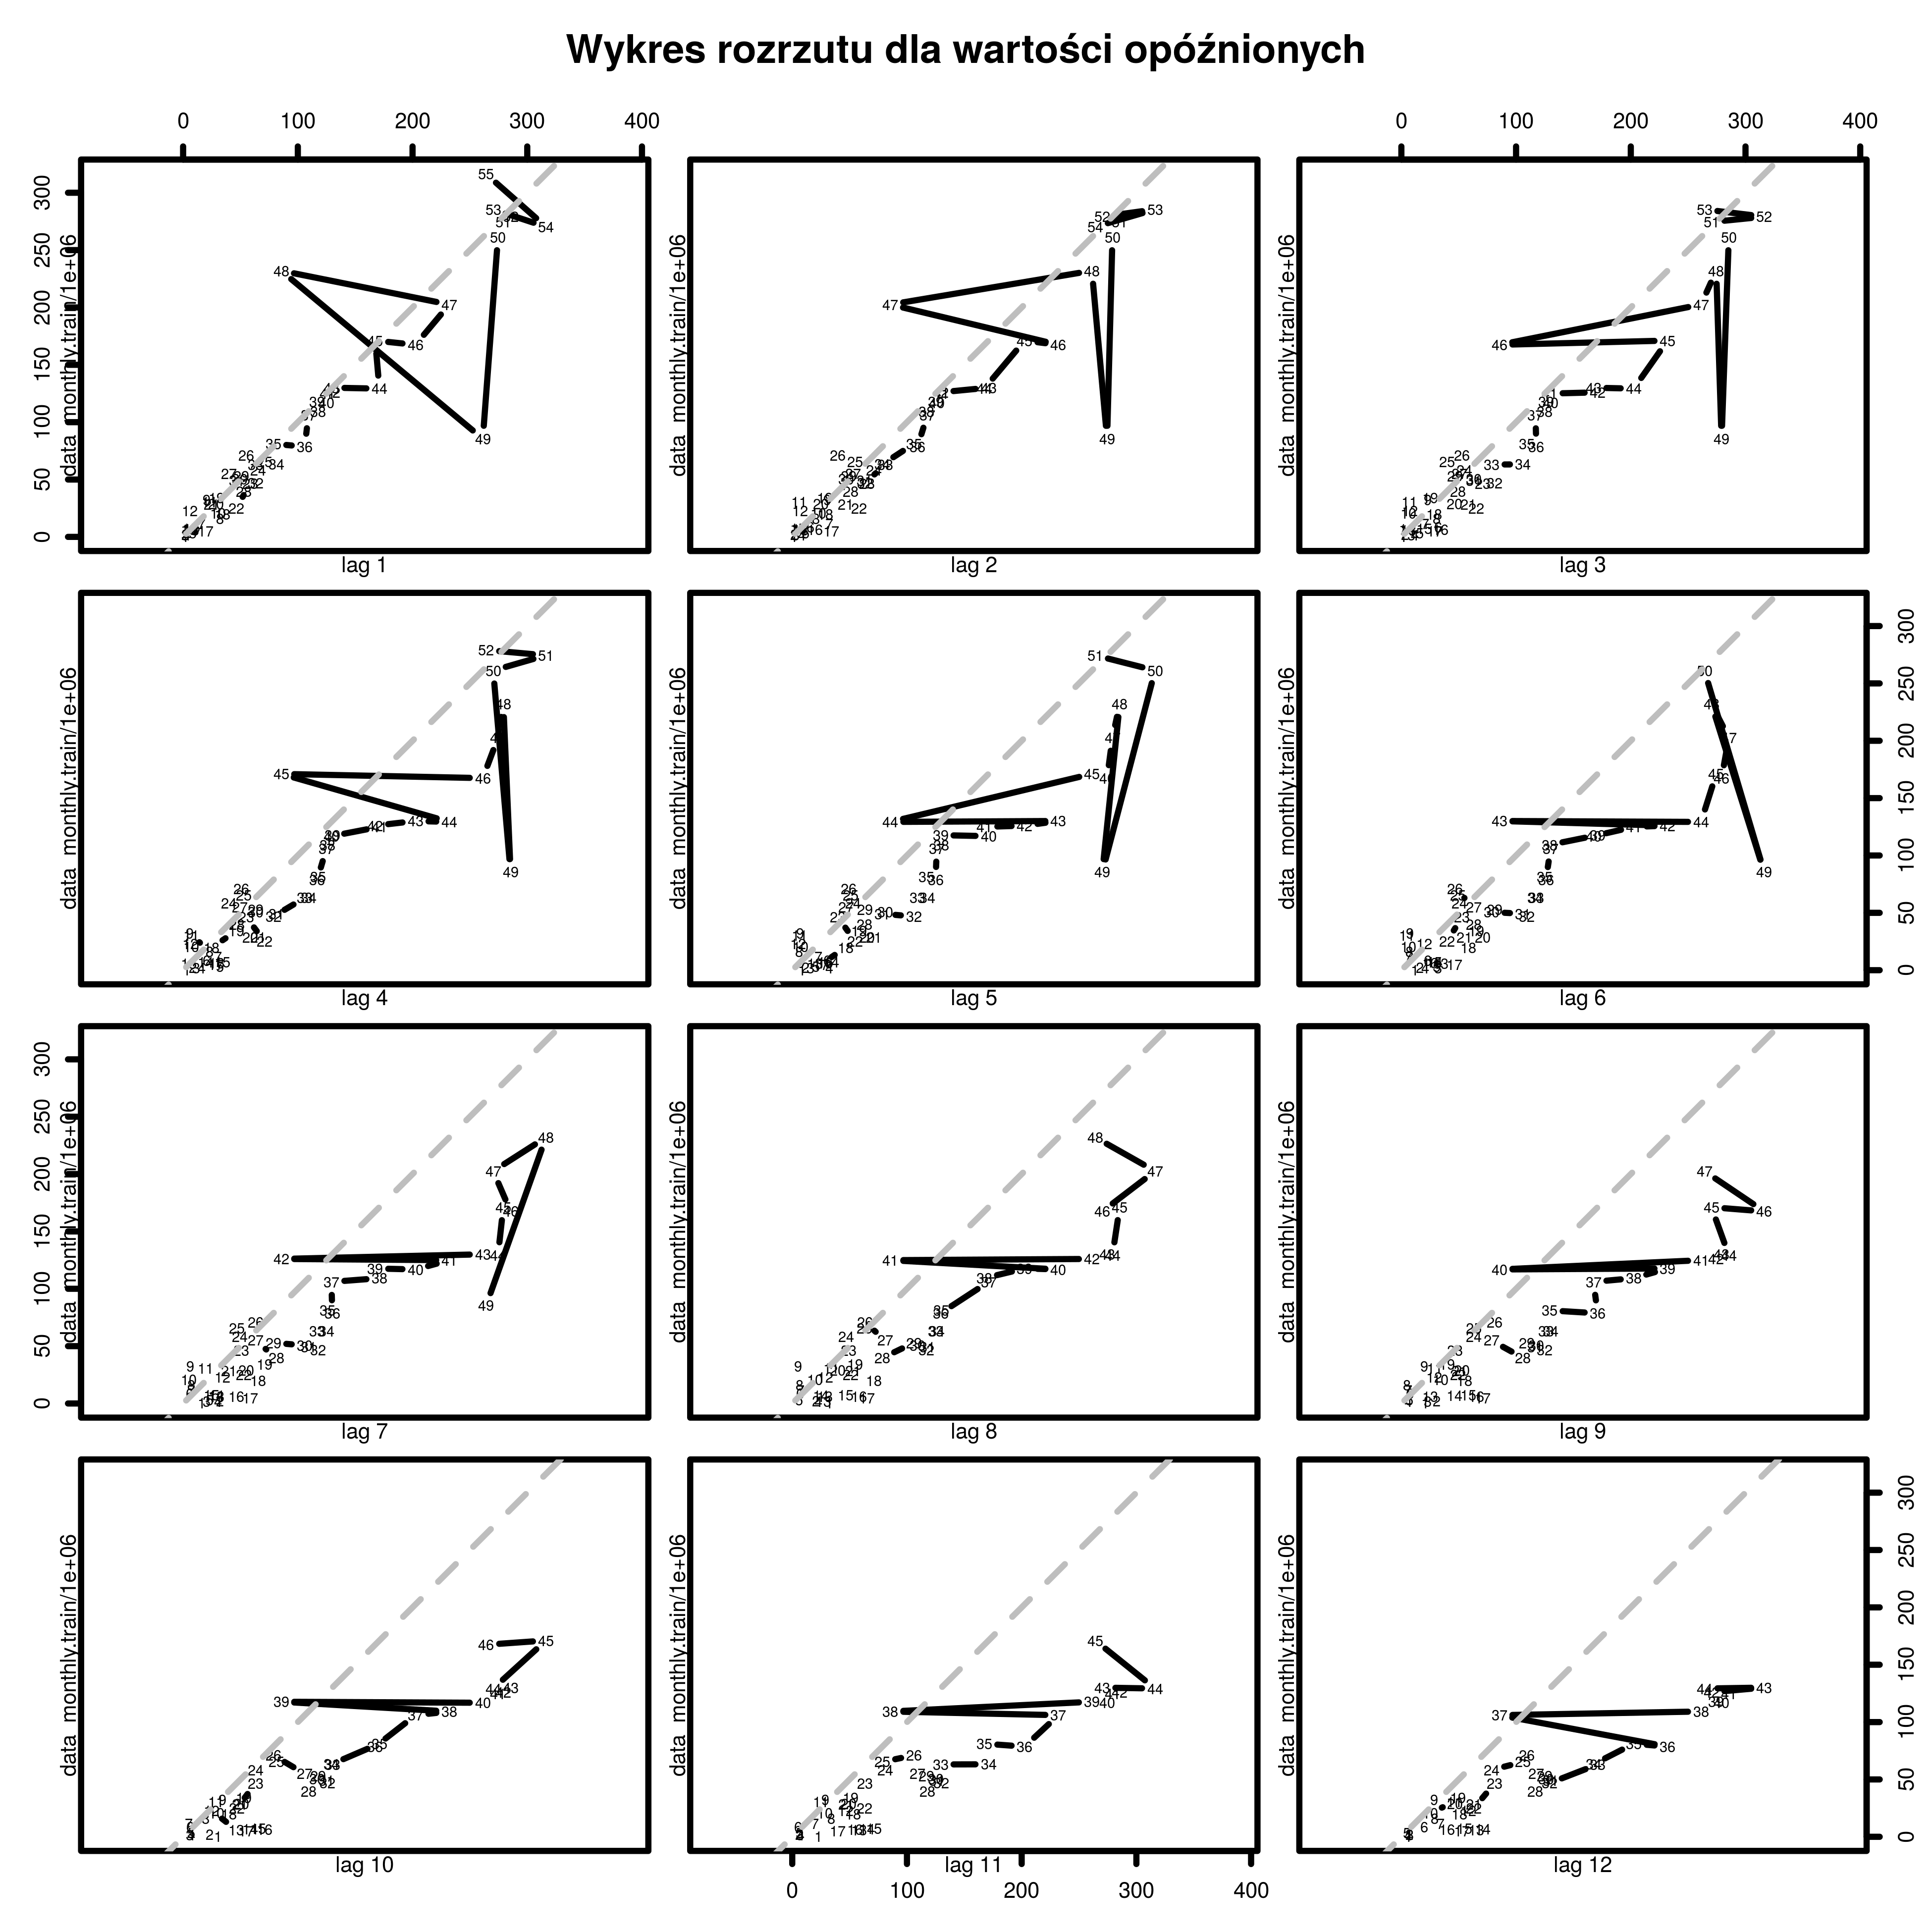
\includegraphics[width=\textwidth]{images/data_monthly_train_opoznienia.png}
    \caption{Wykres rozrzutu dla wartości opóźnionych dla danych miesięcznych analizowanego szeregu czasowego.}
    \label{fig:data_monthly_train_opoznienia}

\end{figure}

\newpage

Wykresy autokorelacji ACF oraz autokorelacji cząstkowej PACF dają nam również informację o tym, że w naszych danych występuje trend wzrostowy poprzez:
\begin{itemize}
\item ACF - Wysoka, dodatnia wartość początkowa, istotna statystycznie zanikająca;
\item PACF - Wartości nie wychodzące poza przedziały ufności.
\end{itemize}

\begin{figure}[h]

    \centering
	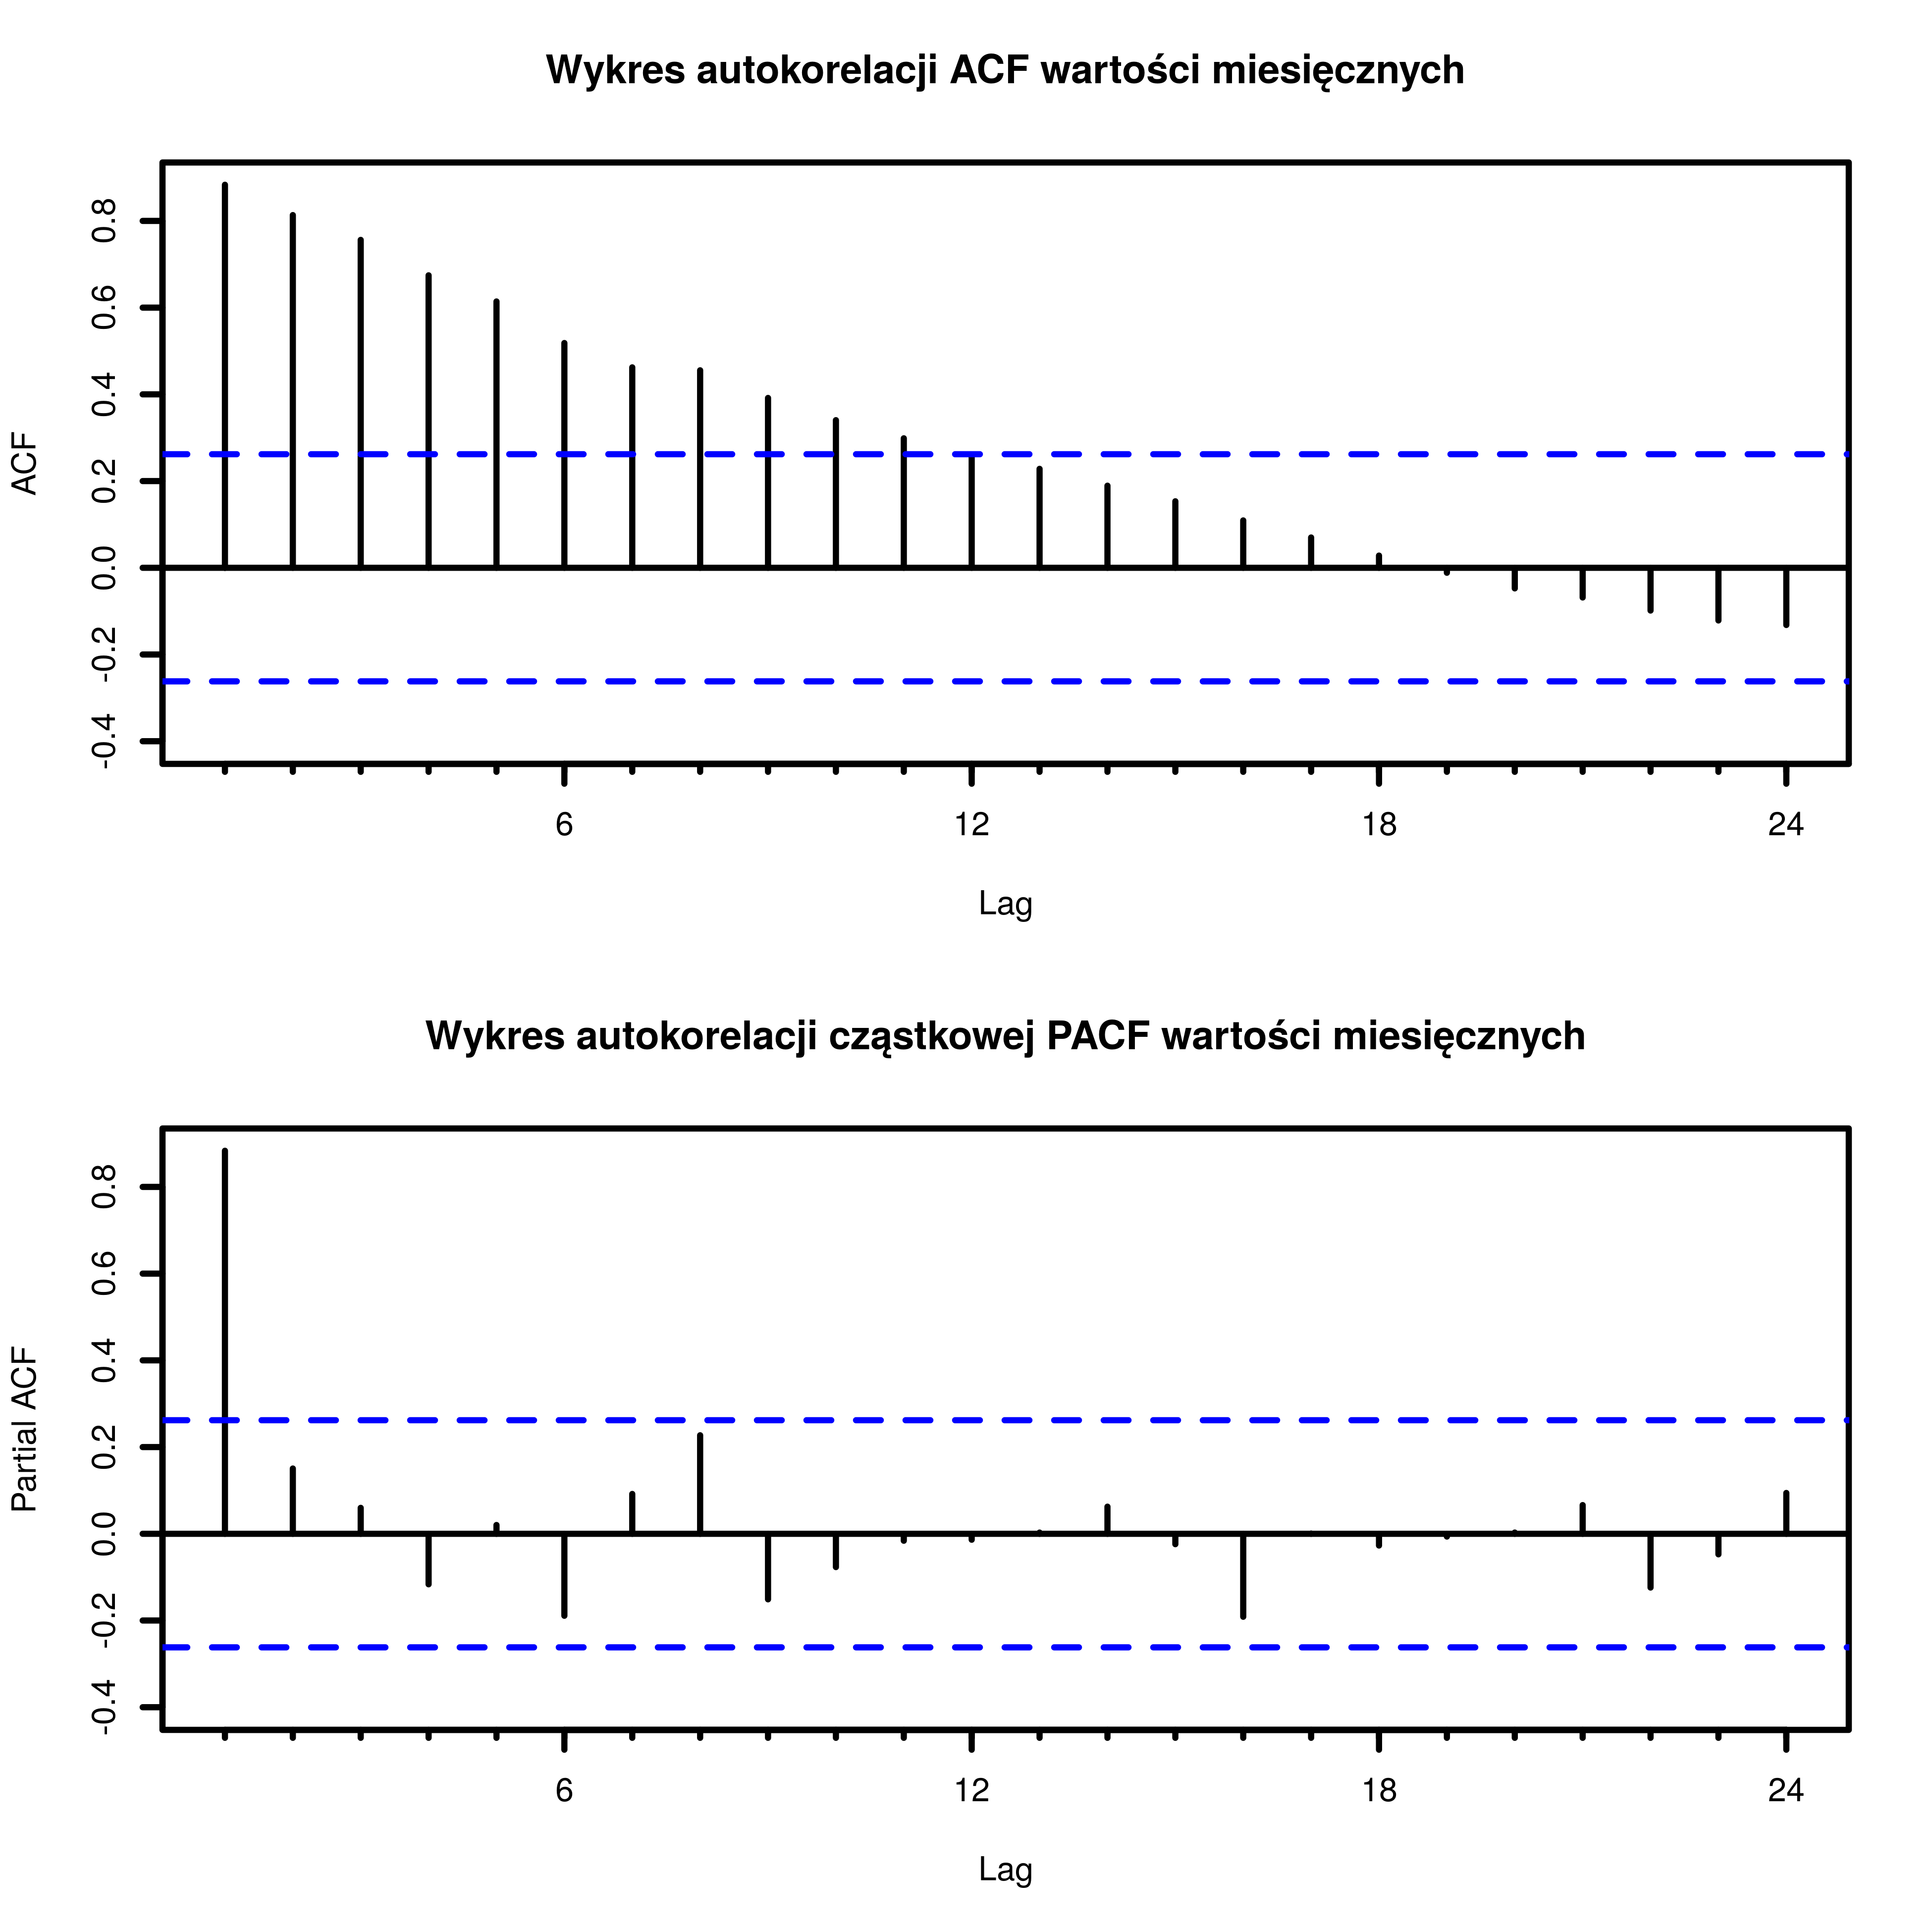
\includegraphics[width=\textwidth]{images/data_monthly_train_wykres_autokorelacji_oraz_czastkowej.png}
    \caption{Wykres autokorelacji (ACF) oraz autokorelacji cząstkowej (PACF) dla danych miesięcznych analizowanego szeregu czasowego.}
    \label{fig:data_monthly_train_wykres_autokorelacji_oraz_czastkowej}

\end{figure}

\newpage

\subsection{Różnicowanie szeregu czasowego}

Za pomocą przekształceń typu: różnicowanie, dekompozycja, transformacja BoxaCoxa. Jesteśmy w stanie pozbyć się trendów oraz sezonowości z naszych danych. Przekształcone dane, w których pozbyliśmy się regularnych tendencji, są znacznie lepsze do analizy oraz interpretacji.

Na przedstawionym poniżej wykresie (Rysunek \ref{fig:data_monthly_train_roznicowanie_z_opoznieniem_jeden}) widoczny jest szereg czasowy, po zastosowaniu różnicowania z opóźnieniem jeden. Po różnicowaniu pozbyliśmy się trendu wzrostowego, co widoczne jest na wykresach autokorelacji ACF oraz autokorelacji cząstkowej PACF. Dzięki nim, możemy wytypować modele. Są to kolejno \textbf{AR(2)}, \textbf{MA(1)}.

\begin{figure}[h]
    \centering
	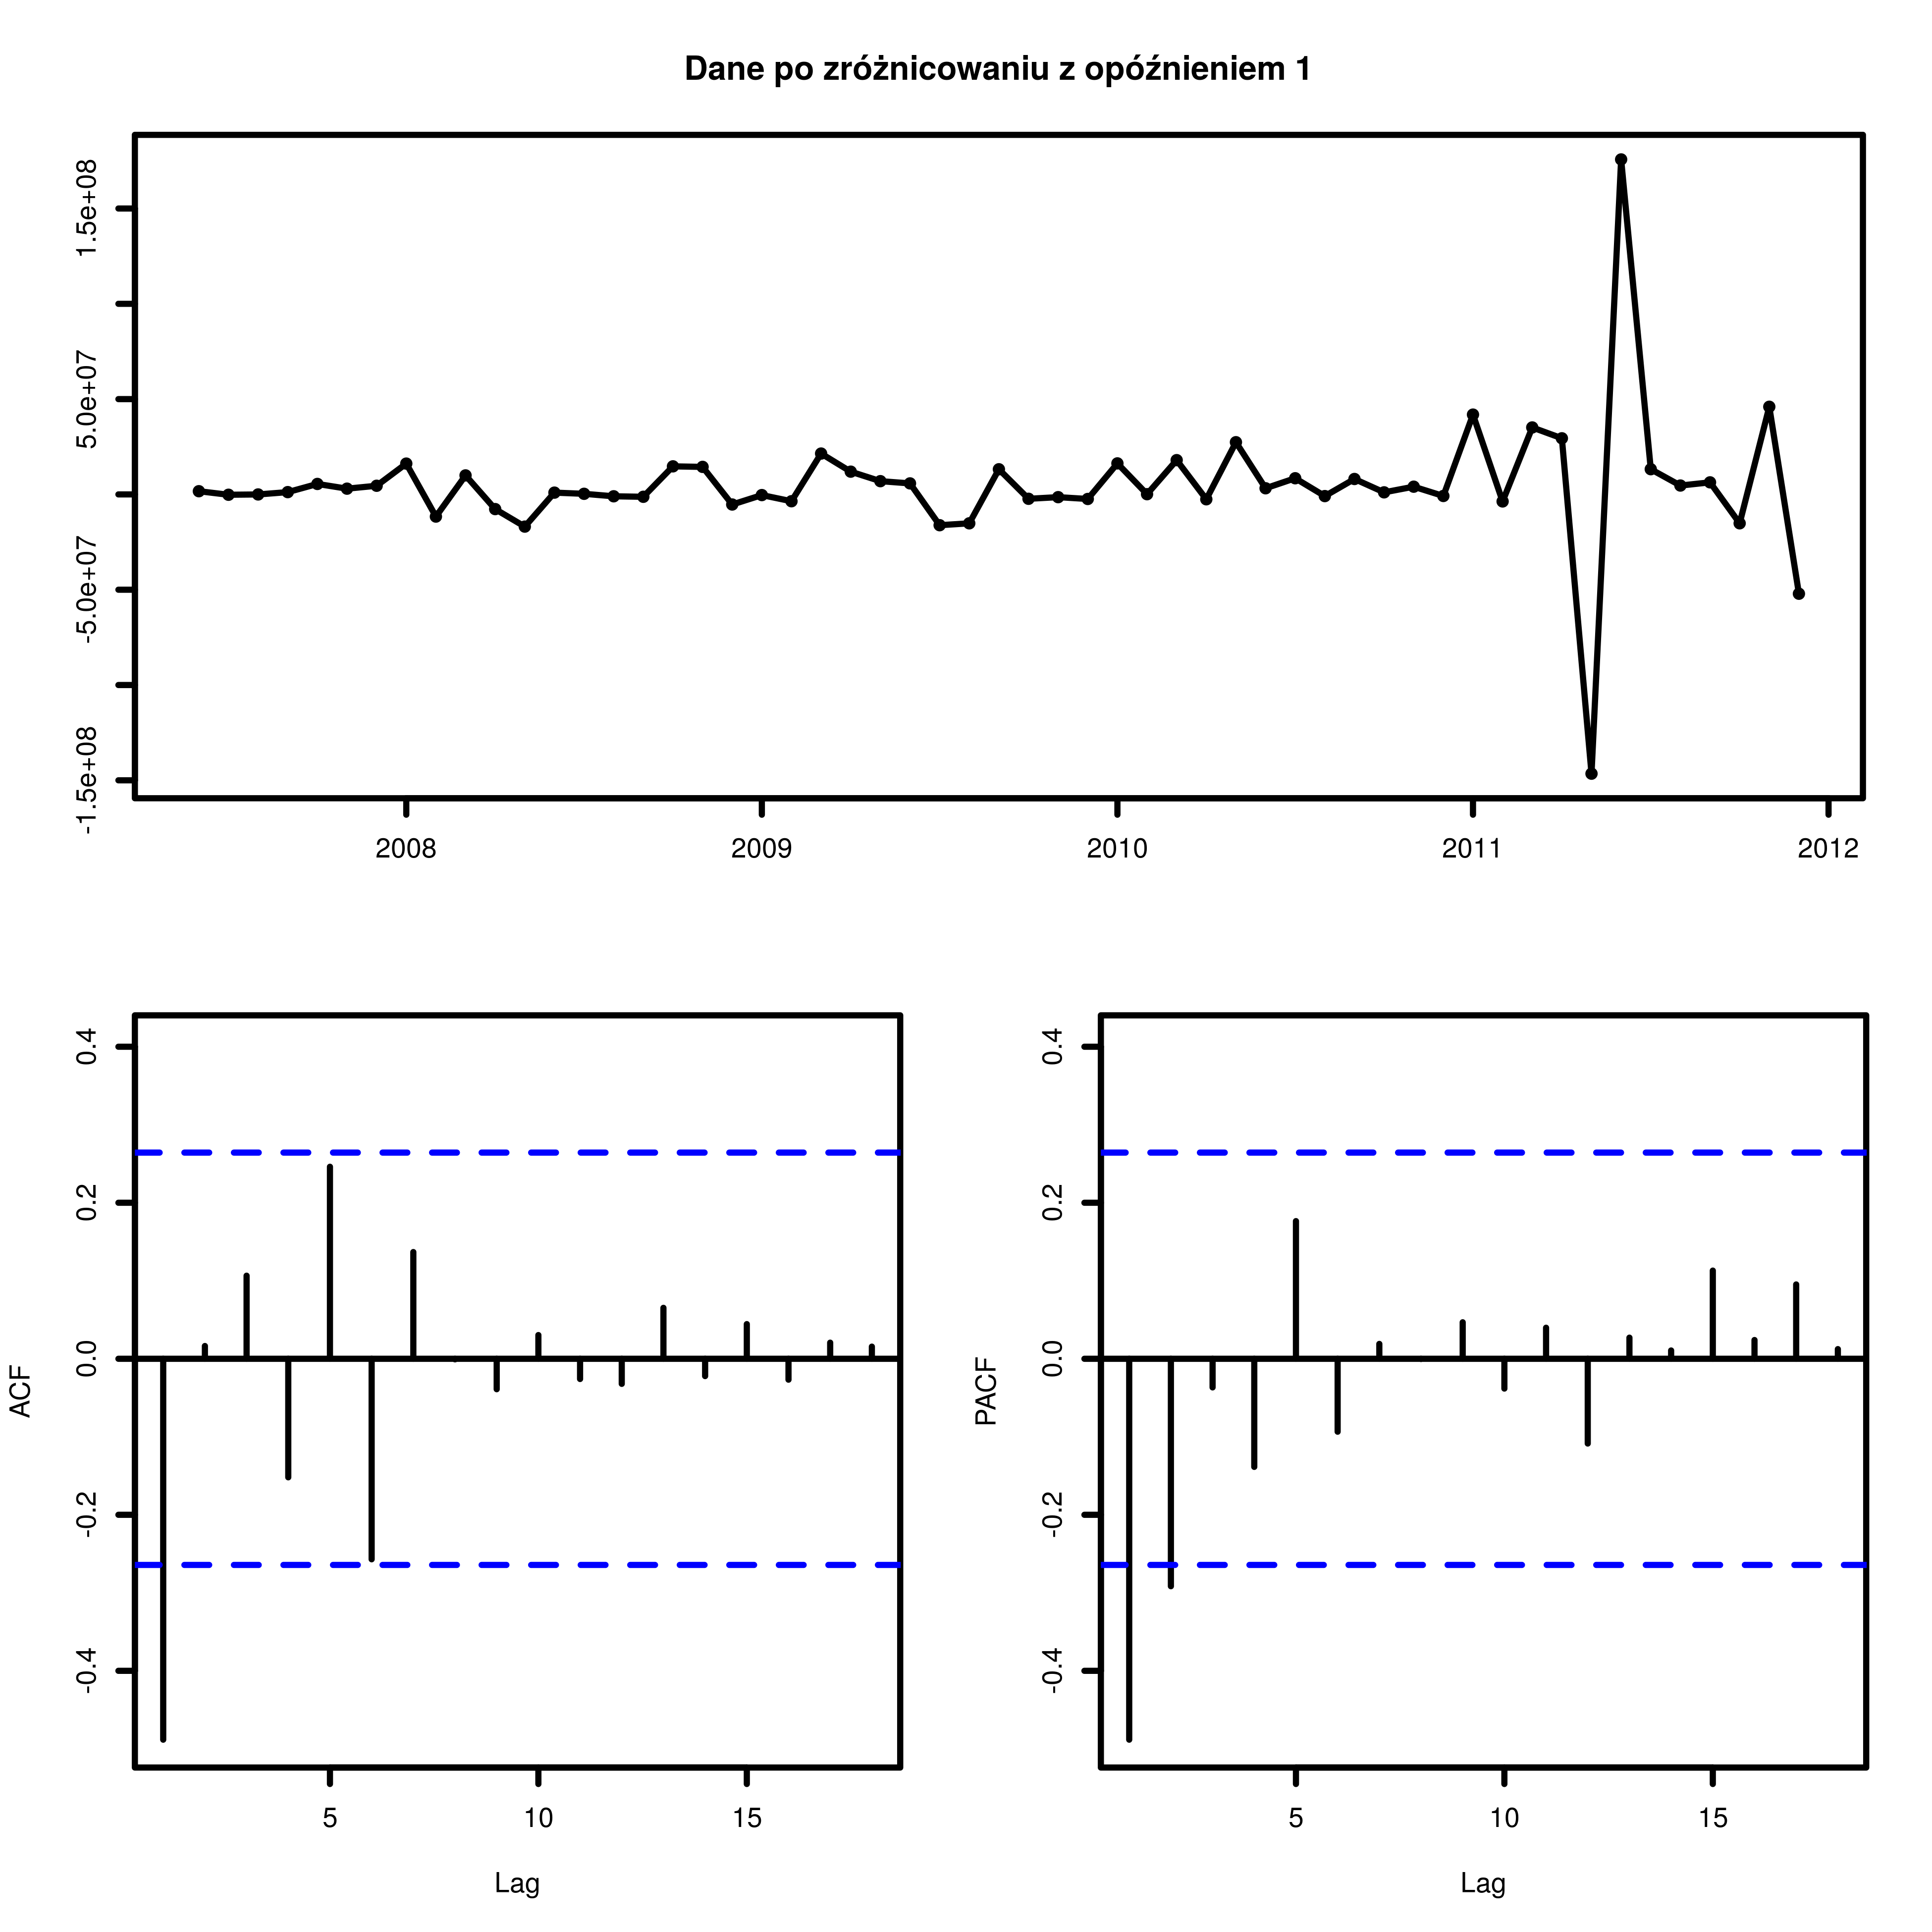
\includegraphics[width=0.9\textwidth]{images/data_monthly_train_roznicowanie_z_opoznieniem_jeden.png}
    \caption{Wykres różnicowania z opóźnieniem jeden dla danych miesięcznych analizowanego szeregu czasowego.}
    \label{fig:data_monthly_train_roznicowanie_z_opoznieniem_jeden}

\end{figure}

\newpage

\section{Diagnostyka wybranych modeli}

Mając na uwadze wybór jak najlepszego modelu, postanowiłem użyć w pakiecie R funkcji \textit{auto.arima}, która wybiera optymalne różnicowanie oraz najlepszy model dla naszych danych. Funkcja ta zwróciła w efekcie model \textbf{MA(2)} z różnicowaniem jeden, czyli taki sam, jaki został przed chwilą wybrany przeze mnie do dalszych analiz.

\subsection{Diagnostyka reszt modeli}

Dla obu testowanych modeli, wykonana została diagnostyka reszt. Na poniższych wykresach (Rysunki \ref{fig:train_monthly_train_AR2_reszty} i \ref{fig:train_monthly_train_MA1_reszty}) nie widać nieregularnych wzorców ani niejednorodności wariancji.

Z ACF i PACF wynika, że nie ma istotnych korelacji

\newpage

\begin{figure}[h]
    \centering
	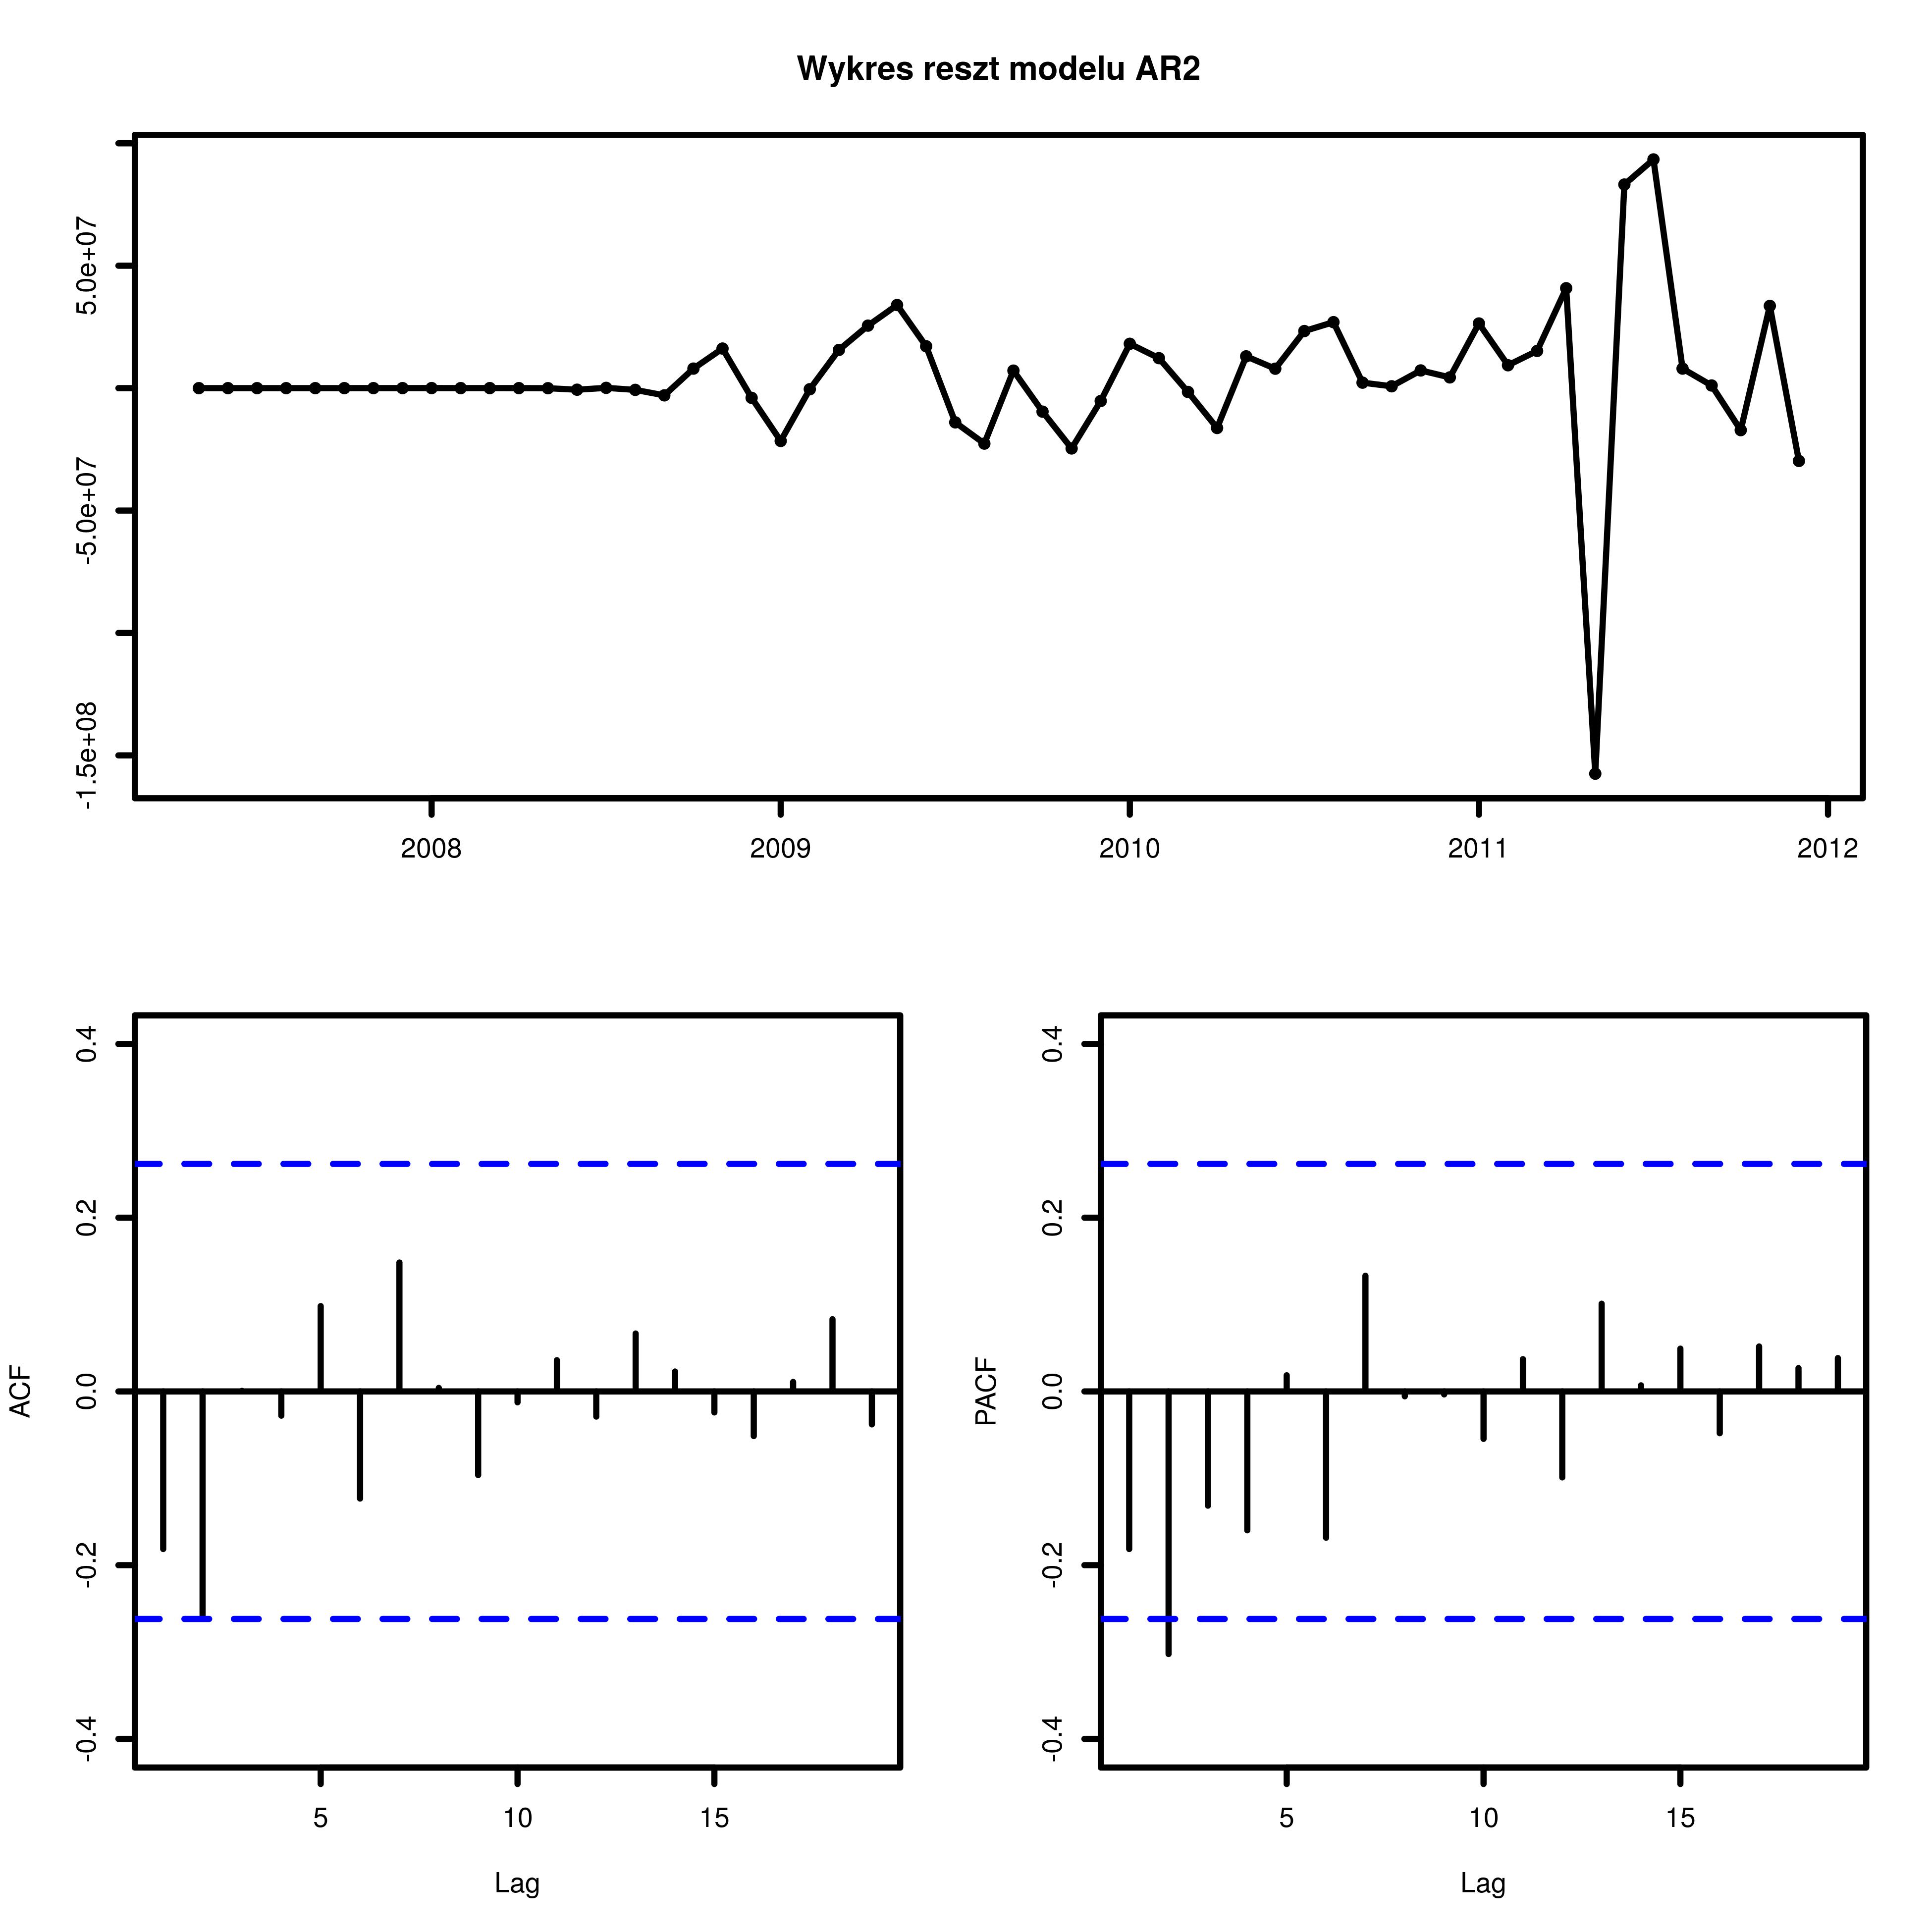
\includegraphics[width=\textwidth]{images/train_monthly_train_AR2_reszty.png}
    \caption{Wykres reszt modelu AR(2).}
    \label{fig:train_monthly_train_AR2_reszty}

\end{figure}

\newpage

\begin{figure}[h]
    \centering
	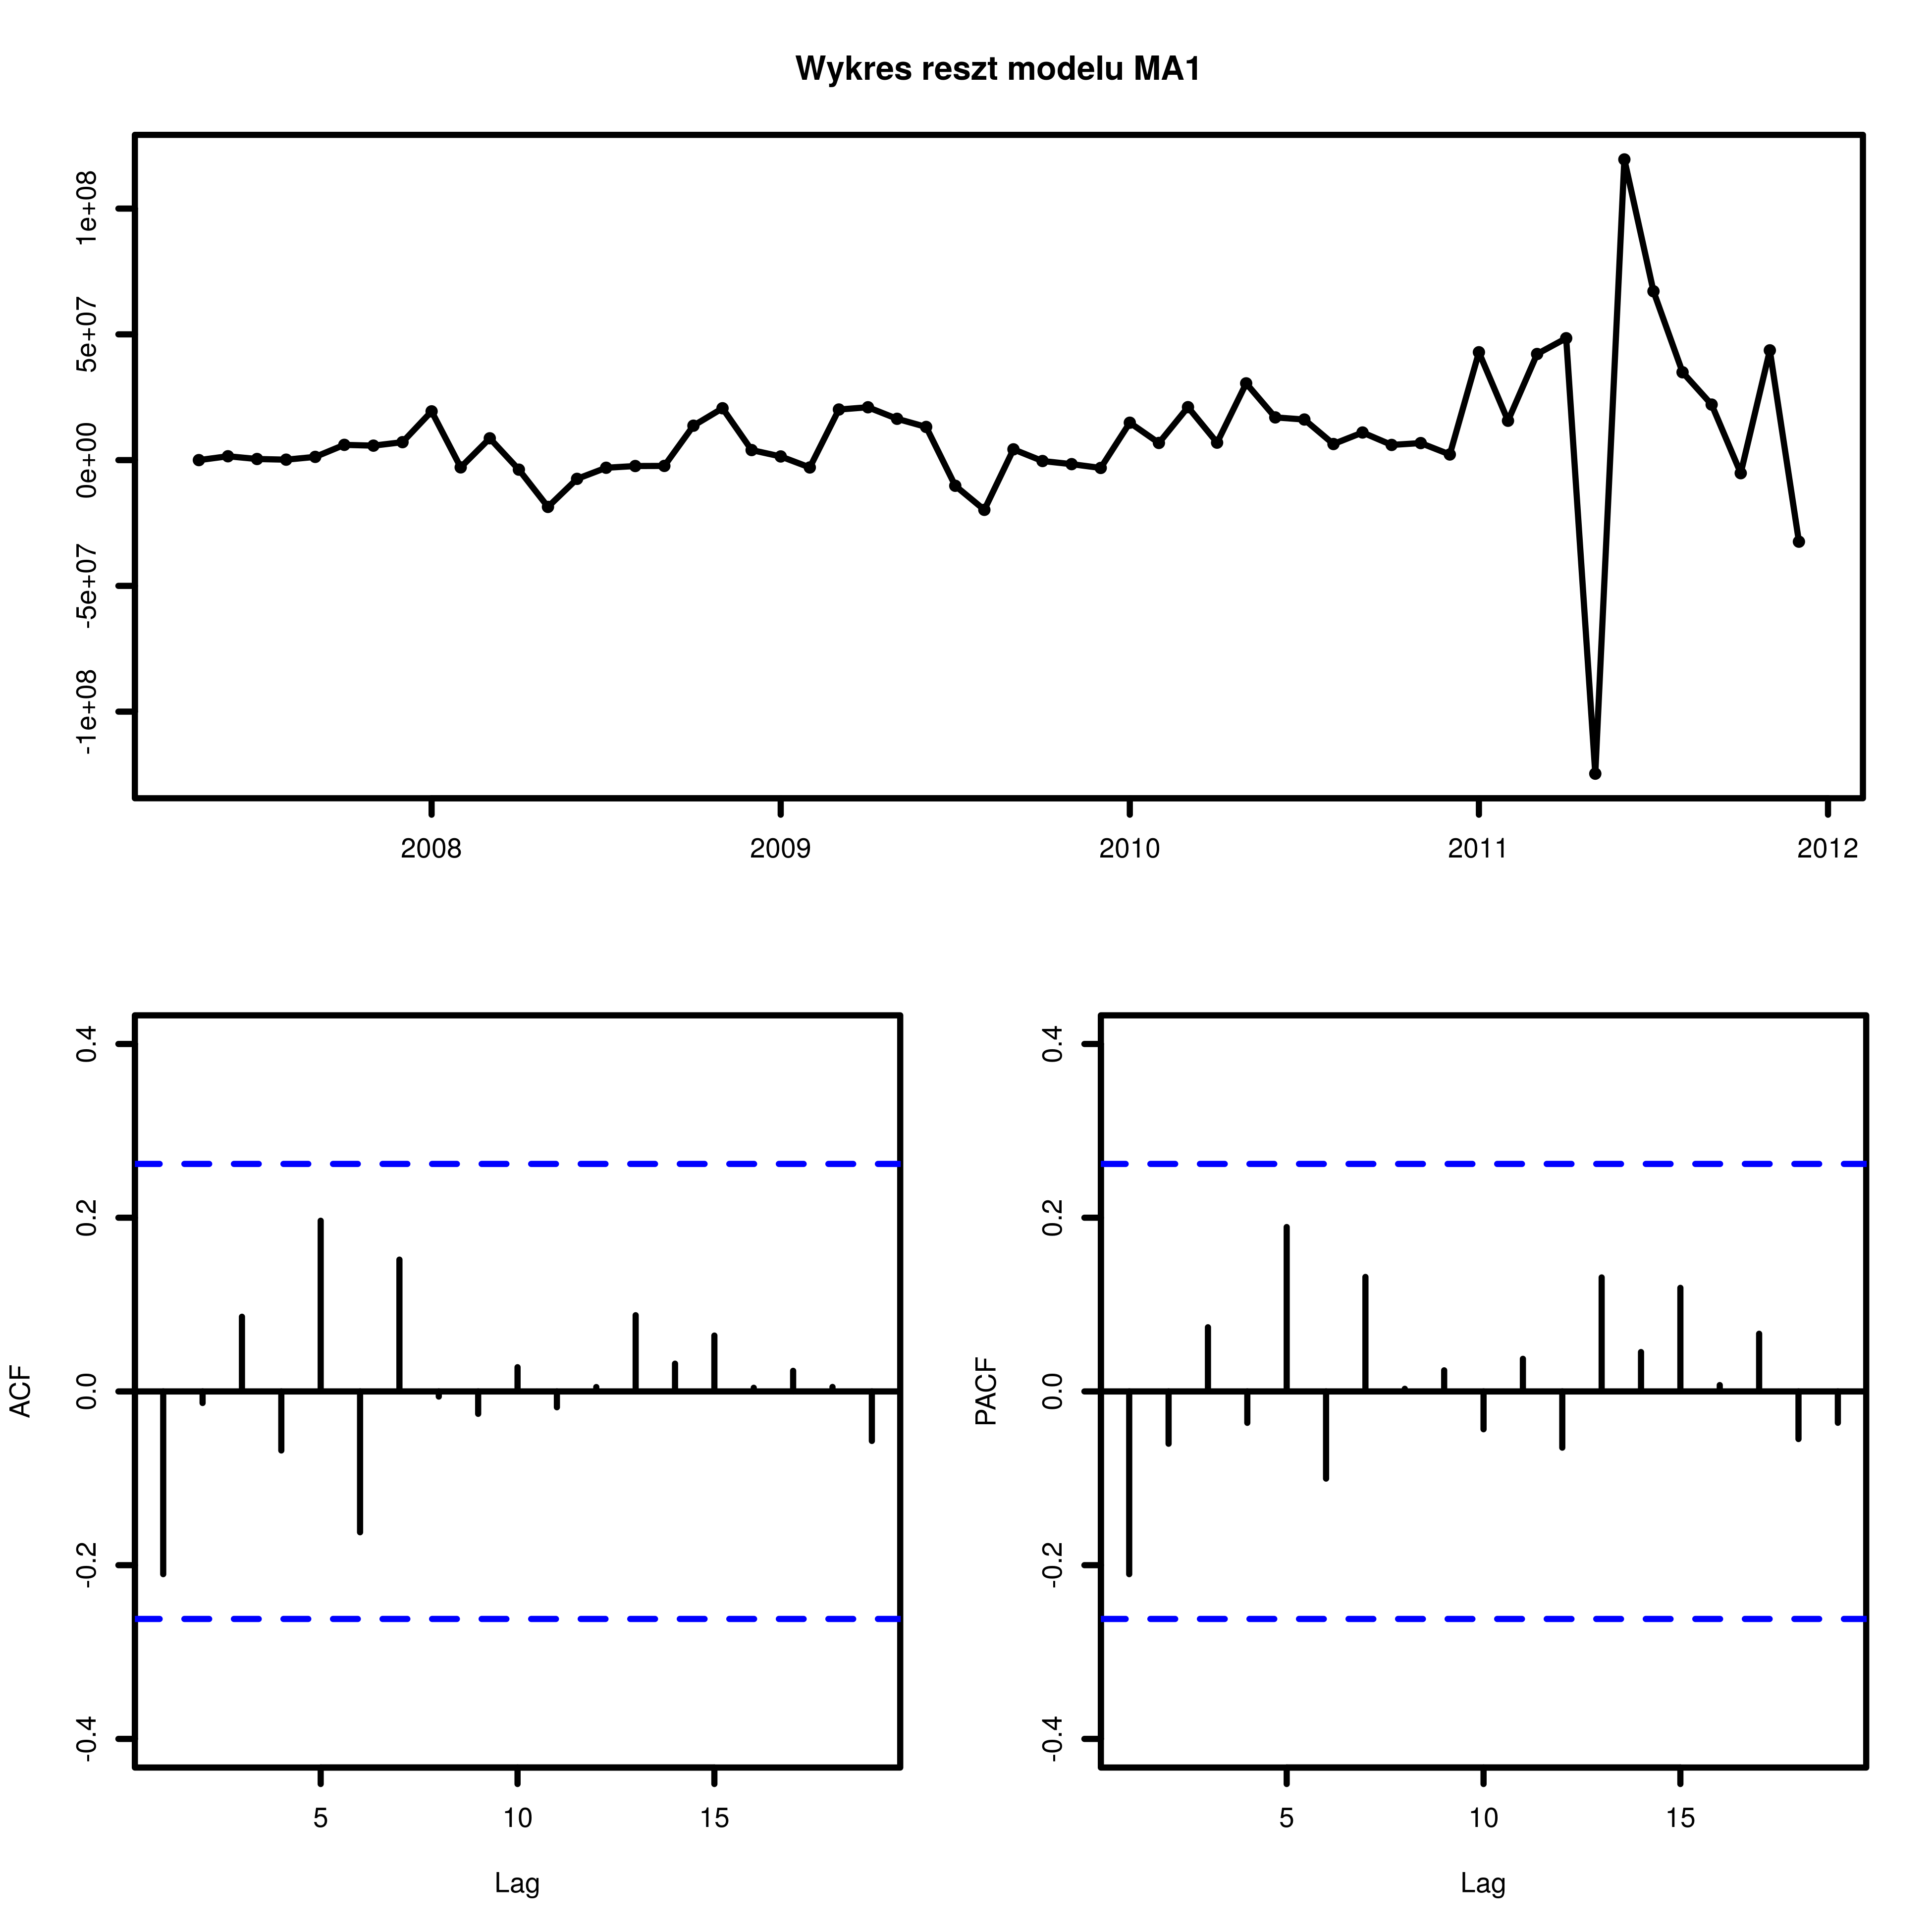
\includegraphics[width=\textwidth]{images/train_monthly_train_MA1_reszty.png}
    \caption{Wykres reszt modelu MA(1).}
    \label{fig:train_monthly_train_MA1_reszty}

\end{figure}

\newpage

\subsection{Prognozowanie}

\subsubsection{ARIMA}
Prognozowanie zostało wykonane dla dwóch modeli ARIMA(2,1,0) oraz ARIMA(0,1,1), które możemy zauważyć na przedstawionych poniżej wykresach Rysunek \ref{fig:prognozy} i \ref{fig:mieszane}. Niestety za pomocą tych wykresów nie jesteśmy w stanie stwierdzić, który model jest lepiej dopasowany. 

W tym celu na stronie \pageref{tab:tabela} wyznaczyłem oceny wykorzystując do tego kryteria błędów predykcji.

\begin{figure}[h]
    \centering
	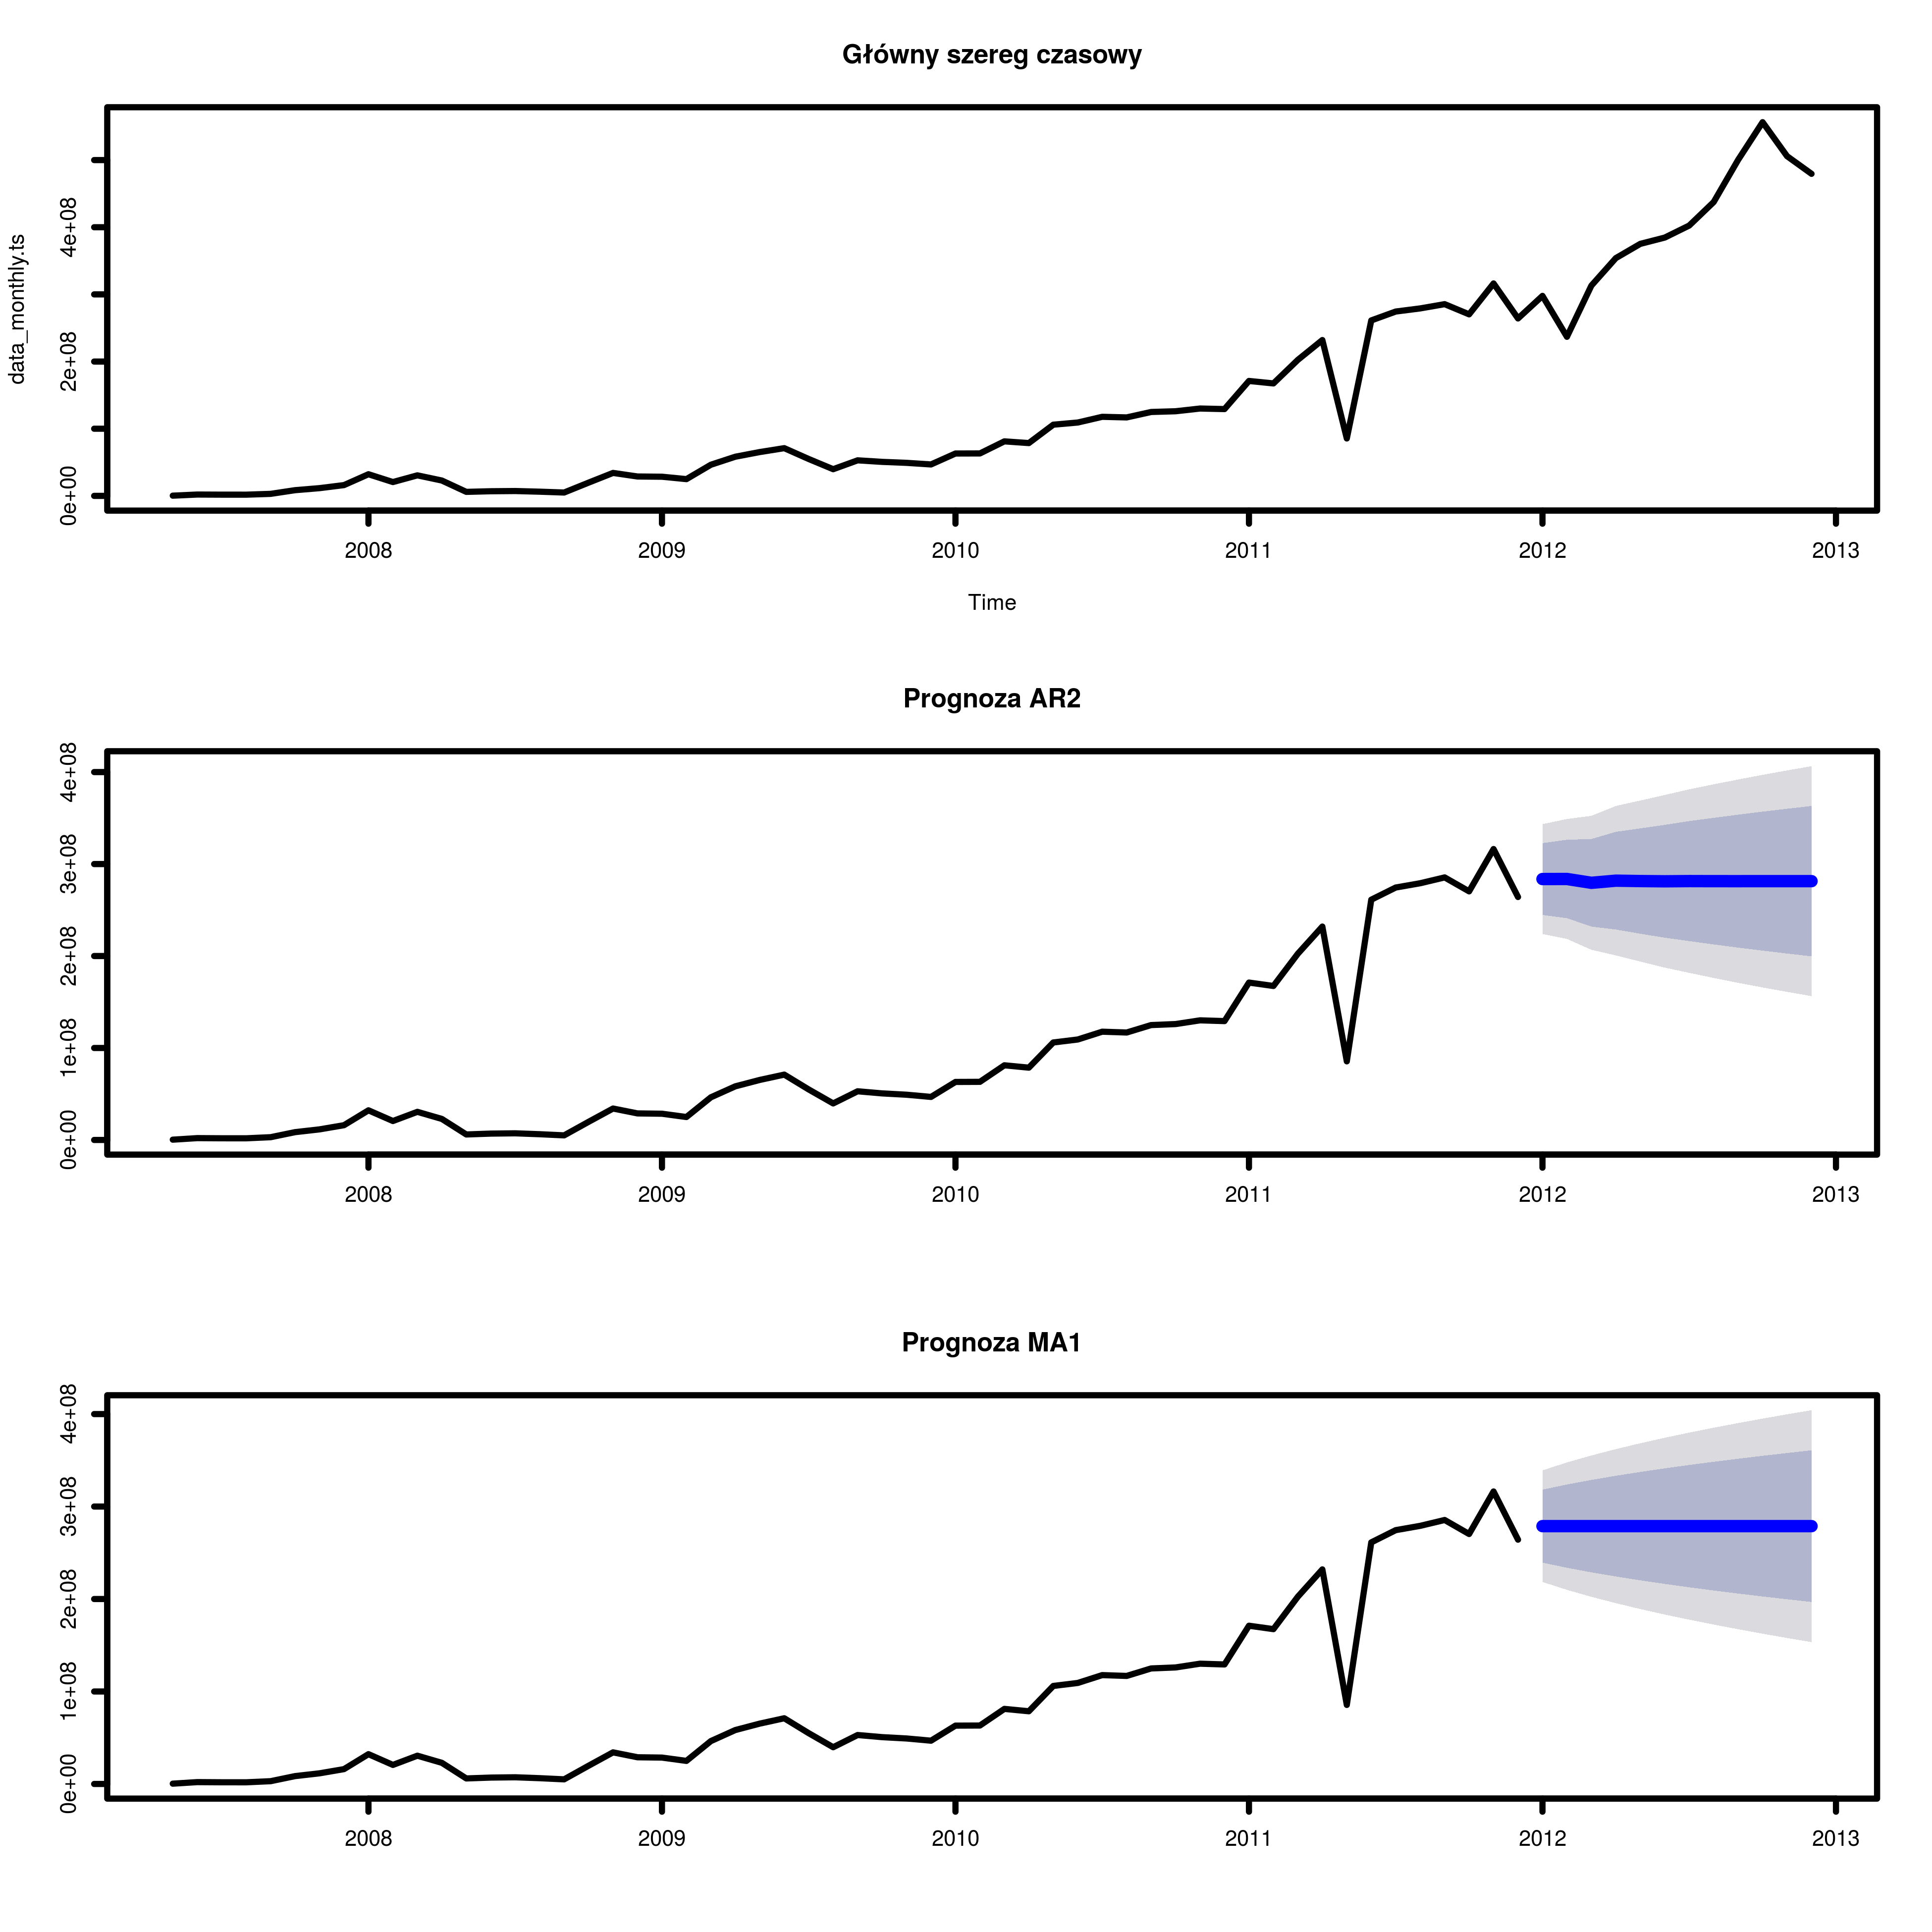
\includegraphics[width=\textwidth]{images/prognozy.png}
    \caption{Analizowany szereg czasowy przedstawiony osobno z wyznaczonymi prognozami dla modeli.}
    \label{fig:prognozy}

\end{figure}

\newpage

\begin{figure}[h]
    \centering
	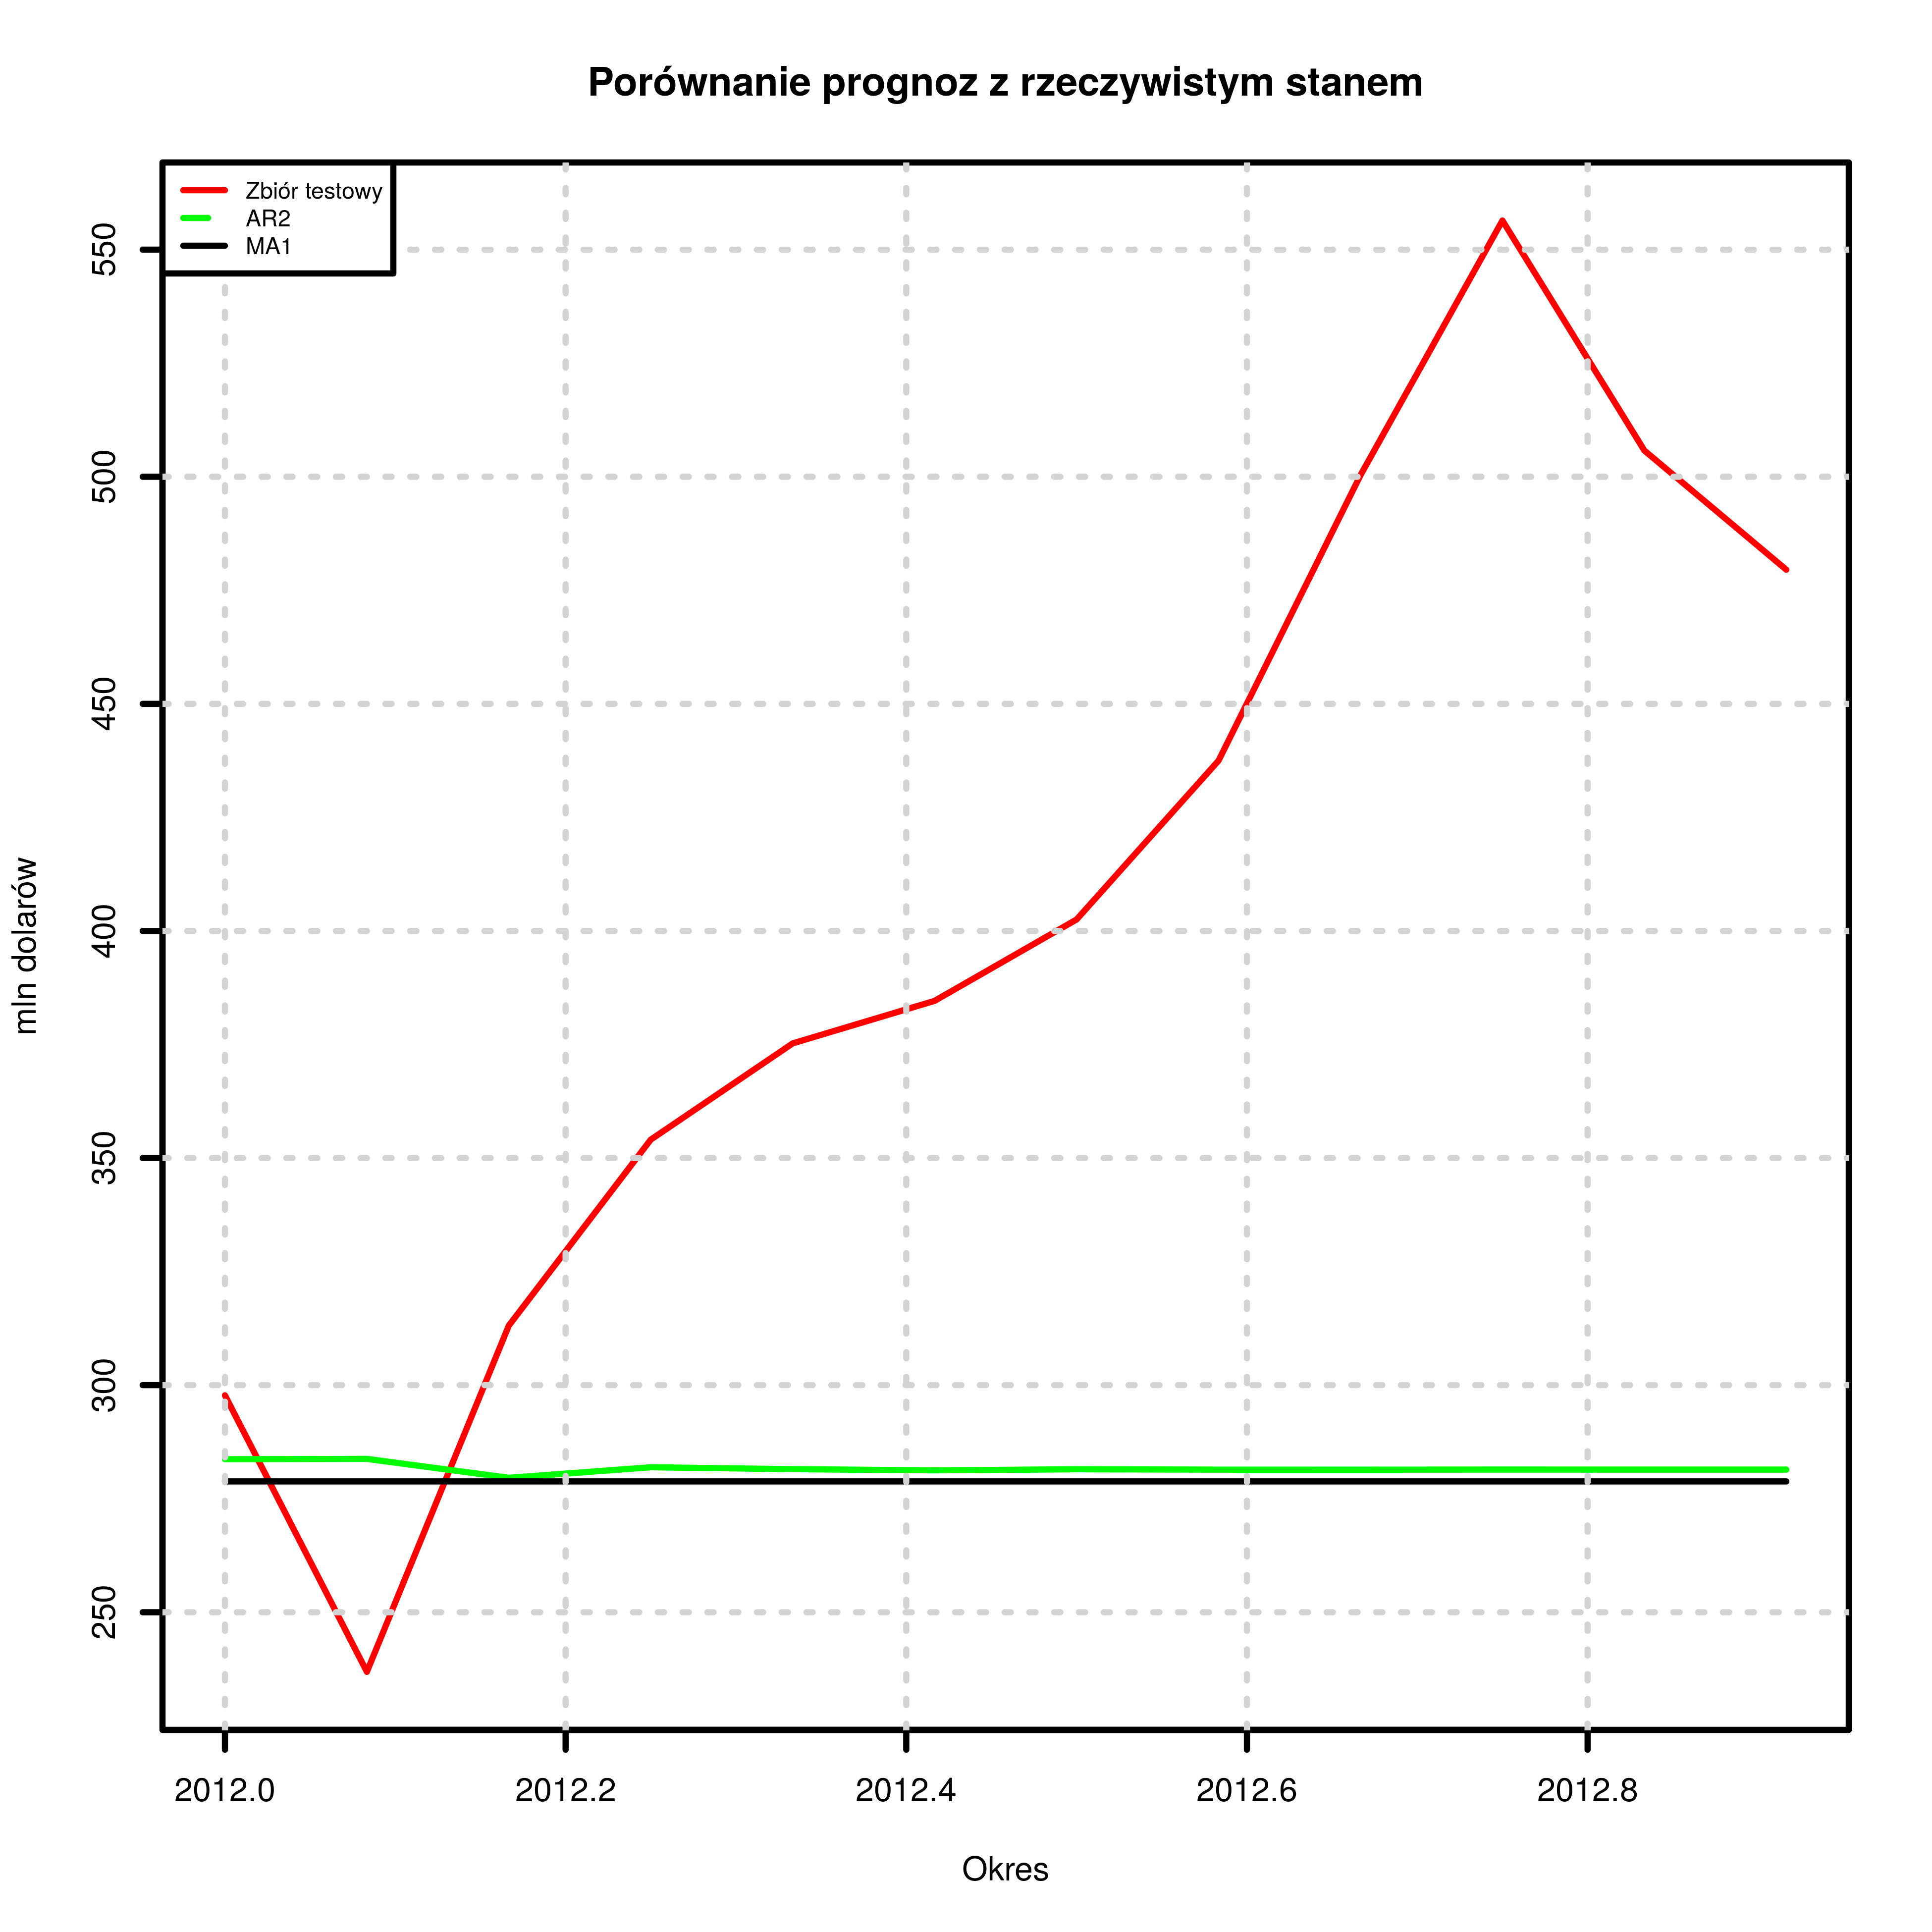
\includegraphics[width=\textwidth]{images/mieszane.png}
    \caption{Przyrównanie analizowanego szeregu czasowego z wyznaczonymi prognozami dla modeli.}
    \label{fig:mieszane}

\end{figure}

\newpage

Wykorzystałem tutaj cztery rodzaje błędów predykcji:

\begin{itemize}
\item \textbf{MAE} (ang. \textit{Mean Absolute Error}) - Średni błąd całkowity;
\item \textbf{RMSE} (ang. \textit{Root Mean Squared Error}) - Błąd średniokwadratowy;
\item \textbf{MAPE} (ang. \textit{Mean Absolute Percentage Error}) - Procent średniego błędu całkowitego;
\item \textbf{MASE} (ang. \textit{Mean Absolute Scaled Error}) - Wyskalowany średni błąd całkowity.
\end{itemize}

W poniższej tabeli widać, że najniższą wartością większości błędów oprócz średniokwadratowego reprezentował sobą model \textbf{MA(1)}.

\begin{center}
\begin{tabular}{l|l|l|l|l|}
\cline{2-5}
                                     & \textbf{MAE} & \textbf{RMSE} & \textbf{MAPE} & \textbf{MASE} \\ \hline
\multicolumn{1}{|l|}{\textbf{AR(2)}} & 17691188.13  & 29636744.22   & 33.49         & 0.29          \\ \hline
\multicolumn{1}{|l|}{\textbf{MA(1)}} & 17645678.03  & 30238184.06   & 32.97         & 0.29          \\ \hline
\end{tabular}
\captionof{table}{Błędy predykcji modeli ARIM.A}
\label{tab:tabela}
\end{center}

\subsubsection{Metoda Holta}

Oceniając jakość modeli, postanowiłem skorzystać z prognozowania metodą Holta, która polega na wygładzaniu wykładniczym. Metoda ta została przeze mnie wybrana, ponieważ w danych występował trend, jednakże nie posiadaliśmy sezonowości.

Prognoza ma charakter liniowy i jest przedstawiona na poniższym wykresie - Rysunek \ref{fig:holt}.


\begin{center}
\begin{tabular}{l|l|l|l|l|}
\cline{2-5}
                                     & \textbf{MAE} & \textbf{RMSE} & \textbf{MAPE} & \textbf{MASE} \\ \hline
\multicolumn{1}{|l|}{\textbf{AR(2)}} & 18451960.86  & 27605036.61   & 76.86         & 0.30          \\ \hline
\end{tabular}
\captionof{table}{Błędy predykcji modelu Holta.}
\label{tab:tabela2}
\end{center}

W powyższej tableli widzimy wcześniej omówione błędy predykcji dla metody Holta. Jak można łatwo zauważyć, metoda ta uzyskała jedynie niższy błąd średniokwadratowy. W ogólnej ocenie modelu wcale nie był on lepszy od wcześniej analizowanych modeli ARIMA.

\clearpage

\begin{figure}[h]
    \centering
	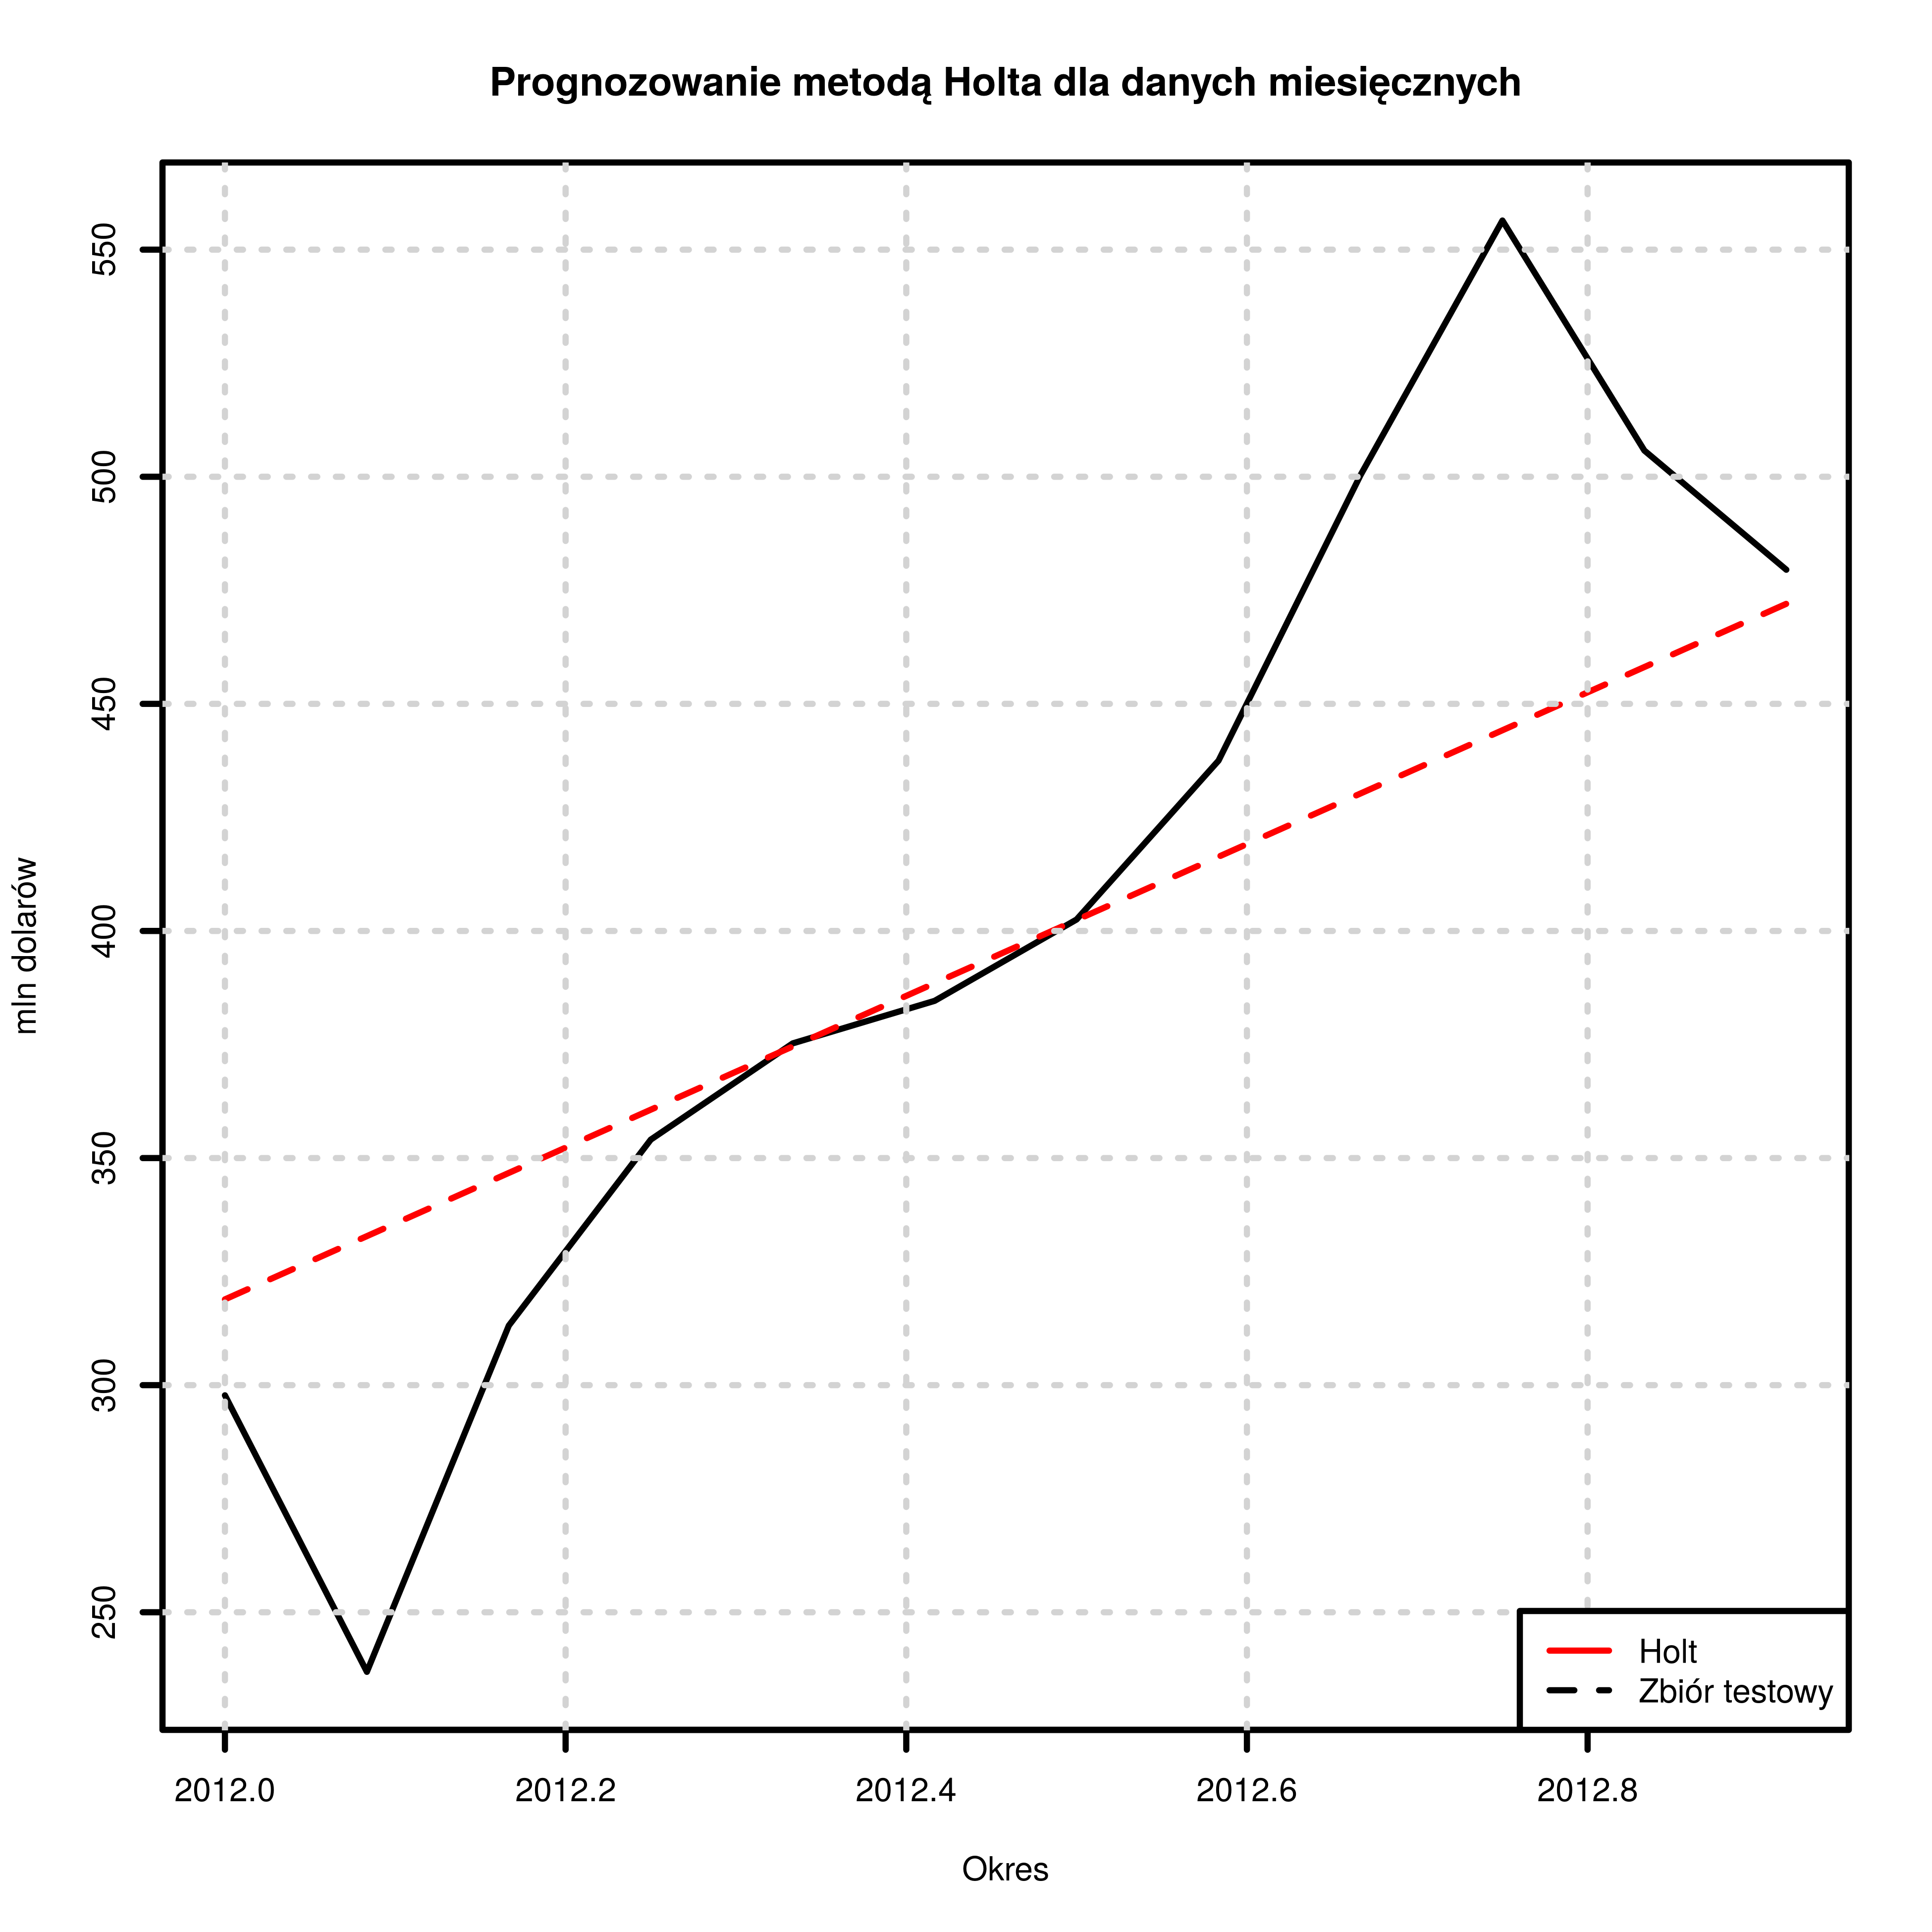
\includegraphics[width=\textwidth]{images/holt.png}
    \caption{Prognoza analizowanego szeregu metodą Holta z jego przyrównaniem do analizowanego szeregu czasowego.}
    \label{fig:holt}

\end{figure}

\newpage

\section{Wnioski}

Wykonane analizy pozwoliły nam wybrać optymalny model do oszacowania prognozy. Przetestowane zostały 3 modele, z czego 2 były oparte na modelu ARIMA oraz jeden na modelu Holta.

Model Holta chociaż z pierwszego punktu widzenia, patrząc na Rysunek \ref{fig:holt}, może wydawać się lepiej dopasowany od modeli ARIMA, tak błędy predykcji (w tym dwa najważniejsze MAPE oraz MASE) wykazały, że jest on gorzej dopasowany.

Z modeli ARIMA najlepiej dopasowanym jest model ARIMA(0,1,1), ponieważ ma niższy procent średniego błędu całkowitego. 

Dopasowany przeze mnie model nie jest idealny, możliwe, że jest to spowodowane moim błędem w ocenie lub za małą grupą uczącą się, dzięki której moglibyśmy wyznaczyć dokładniejszy model.



\clearpage

\listoffigures

\listoftables

\end{document}
